% BDC223 Lecture 9a: Nutrient uptake. Slides with TikZ diagrams and Python graphs (figures/make_figures.py).
% Each frame replaces one image in L09a-nutrient_uptake.qmd; the "% pos NN" comment before a frame names
% the qmd image position it fills (see build.sh). Diagrams labelled "schematic" are conceptual. Graph values
% come from Smit (2002) Bot. Mar. 45: 196-209 (Tables I-III), Epstein (1972) and DeBoer (1981).
\documentclass[aspectratio=169,11pt]{beamer}
\usepackage[sfdefault,lining]{FiraSans}
\usepackage{amsmath}
\usefonttheme{professionalfonts}
\usepackage{firamath-otf}
\setmathrm{Fira Sans}
\usepackage{tikz}
\usepackage{pgfplots}
\usepackage{array}
\usepackage{graphicx}
\graphicspath{{figures/}}
\pgfplotsset{compat=1.18}
\usetikzlibrary{arrows.meta,positioning,calc,shapes.geometric,decorations.pathmorphing}

\definecolor{ink}{HTML}{1F2A37}
\definecolor{accent}{HTML}{0F766E}
\definecolor{sea}{HTML}{1D4E89}
\definecolor{grey}{HTML}{6B7280}
\definecolor{leaf}{HTML}{3F8F2F}
\definecolor{warm}{HTML}{B45309}
\definecolor{hot}{HTML}{B91C1C}
\definecolor{sand}{HTML}{F2B84B}
\setbeamercolor{frametitle}{fg=white,bg=ink}
\setbeamercolor{normal text}{fg=ink,bg=white}
\setbeamercolor{itemize item}{fg=accent}
\setbeamercolor{itemize subitem}{fg=accent}
\setbeamertemplate{itemize item}{\small$\blacktriangleright$}
\setbeamertemplate{itemize subitem}{\footnotesize\textendash}
\setbeamertemplate{navigation symbols}{}
\setbeamerfont{frametitle}{size=\Large,series=\bfseries}
\setbeamertemplate{frametitle}{%
  \nointerlineskip
  \begin{beamercolorbox}[wd=\paperwidth,ht=2.4em,dp=0.9em,leftskip=1.2em]{frametitle}
    \insertframetitle
  \end{beamercolorbox}}
\setbeamertemplate{footline}{%
  \hbox to \paperwidth{\hspace{1.2em}\color{grey}\tiny BDC223 Plant Ecophysiology \textbar{} Lecture 9a: Nutrient Uptake\hfill\insertframenumber\hspace{1.2em}}\vspace{0.6em}}
\setlength{\leftmargini}{1.4em}
\setbeamerfont{normal text}{size=\footnotesize}
\setbeamerfont{itemize/enumerate body}{size=\footnotesize}
\setbeamerfont{itemize/enumerate subbody}{size=\footnotesize}
\newcommand{\colsize}{\footnotesize}
\hyphenpenalty=10000
\newcommand{\fignote}[1]{\par\vspace{2pt}{\color{grey}\scriptsize #1}}
\newcommand{\twocol}[2]{%
  \begin{columns}[c,onlytextwidth]
    \begin{column}{0.44\textwidth}\colsize #1\end{column}
    \begin{column}{0.54\textwidth}\centering #2\end{column}
  \end{columns}}
\tikzset{
  card/.style={draw=#1, very thick, rounded corners, fill=#1!7, align=flush left, inner sep=5pt},
  flow/.style={draw=#1, thick, rounded corners, fill=#1!8, align=center, inner sep=4pt, font=\scriptsize},
  arr/.style={-{Stealth[length=2.2mm]}, thick, grey}}


\begin{document}
% Part 1: qmd image positions 07-45. Content from old slide P-1, qualified by the lecture prose.
\tikzset{el/.style={draw=#1, thick, fill=#1!12, minimum width=0.85cm, minimum height=0.85cm, rounded corners=2pt}}

% pos 07
\begin{frame}{Seaweeds take up nutrients across the whole thallus}
\twocol{
\begin{itemize}
  \item Algae, like land plants, need nutrients for persistence, growth and reproduction
  \item Seaweeds are bathed in the medium that supplies them (intertidal species for most of the time)
  \item Uptake occurs across the thallus surface: no roots are needed
  \item Surface area to volume ratio therefore matters (Lecture 2)
  \item Many land plants rely on mycorrhizae or root nodules; seaweeds have their own uptake systems
\end{itemize}}{
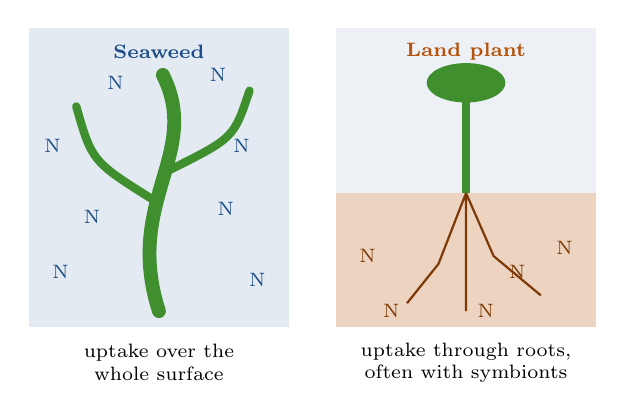
\begin{tikzpicture}[font=\scriptsize]
  \fill[sea!12] (-3.6,-1.2) rectangle (-0.3,2.6);
  \node[font=\scriptsize\bfseries, sea] at (-1.95,2.3) {Seaweed};
  \draw[leaf, line width=5pt, line cap=round] (-1.95,-1.0) .. controls (-2.4,0.4) and (-1.4,1.0) .. (-1.9,2.0);
  \draw[leaf, line width=3pt, line cap=round] (-2.0,0.4) .. controls (-2.8,0.9) .. (-3.0,1.6);
  \draw[leaf, line width=3pt, line cap=round] (-1.8,0.8) .. controls (-1.0,1.2) .. (-0.8,1.8);
  \foreach \x/\y in {-3.2/-0.5,-2.8/0.2,-1.1/0.3,-0.7/-0.6,-2.5/1.9,-1.2/2.0,-3.3/1.1,-0.9/1.1}
    \node[font=\scriptsize, sea] at (\x,\y) {N};
  \fill[warm!25] (0.3,-1.2) rectangle (3.6,0.5);
  \fill[sea!8] (0.3,0.5) rectangle (3.6,2.6);
  \node[font=\scriptsize\bfseries, warm] at (1.95,2.3) {Land plant};
  \draw[leaf, line width=3pt] (1.95,0.5) -- (1.95,1.9);
  \fill[leaf] (1.95,1.9) ellipse (0.5 and 0.25);
  \draw[warm!70!black, thick] (1.95,0.5) -- (1.6,-0.4) -- (1.2,-0.9) (1.95,0.5) -- (2.3,-0.3) -- (2.9,-0.8) (1.95,0.5) -- (1.95,-1.0);
  \foreach \x/\y in {0.7/-0.3,1.0/-1.0,2.6/-0.5,3.2/-0.2,2.2/-1.0}
    \node[font=\scriptsize, warm!70!black] at (\x,\y) {N};
  \node[font=\scriptsize, align=center, text width=3.1cm] at (-1.95,-1.65) {uptake over the whole surface};
  \node[font=\scriptsize, align=center, text width=3.1cm] at (1.95,-1.65) {uptake through roots, often with symbionts};
\end{tikzpicture}
\fignote{Schematic.}}
\end{frame}

% pos 08
\begin{frame}{Essential and beneficial nutrients}
\twocol{
\begin{itemize}
  \item Much of what we know about algal nutrition comes from work on culture media between the 1930s and 1970s
  \item These studies identified \textbf{essential} and \textbf{beneficial} nutrients
  \item Beneficial nutrients promote growth or function but are not required to complete the life cycle
\end{itemize}}{
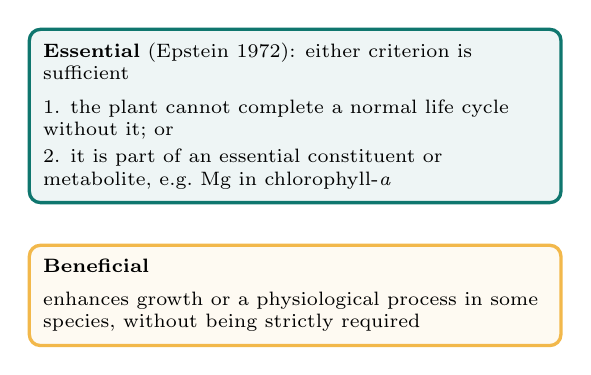
\begin{tikzpicture}[font=\scriptsize]
  \node[card=accent, text width=6.4cm] (e) {\textbf{Essential} (Epstein 1972): either criterion is sufficient\\[4pt]
    1. the plant cannot complete a normal life cycle without it; or\\[2pt]
    2. it is part of an essential constituent or metabolite, e.g.\ Mg in chlorophyll-\textit{a}};
  \node[card=sand, text width=6.4cm, below=0.5cm of e] {\textbf{Beneficial}\\[4pt] enhances growth or a physiological process in some species, without being strictly required};
\end{tikzpicture}}
\end{frame}

% pos 09
\begin{frame}{A second test of essentiality}
\twocol{
\begin{itemize}
  \item An alternative definition sets three conditions
  \item The first overlaps with Epstein's life-cycle criterion
  \item An essential role may be structural, metabolic or as an enzyme cofactor
\end{itemize}}{
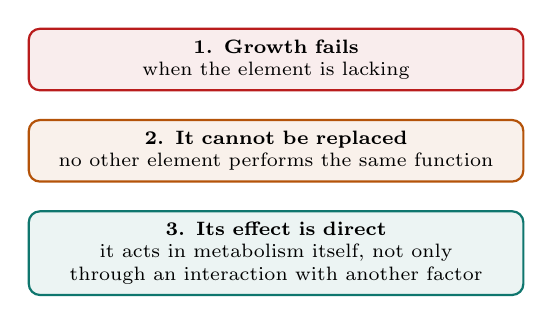
\begin{tikzpicture}[font=\scriptsize]
  \node[flow=hot, text width=6.0cm] (a) {\textbf{1. Growth fails}\\ when the element is lacking};
  \node[flow=warm, text width=6.0cm, below=0.35cm of a] (b) {\textbf{2. It cannot be replaced}\\ no other element performs the same function};
  \node[flow=accent, text width=6.0cm, below=0.35cm of b] (c) {\textbf{3. Its effect is direct}\\ it acts in metabolism itself, not only through an interaction with another factor};
\end{tikzpicture}}
\end{frame}

% pos 10
\begin{frame}{Macronutrients and micronutrients}
\twocol{
\begin{itemize}
  \item Classified by the quantity in tissue or the amount needed in nutrient solutions
  \item Quantity says nothing about importance: every essential element is required
  \item Macronutrients: mainly structural; some are also regulatory (e.g.\ Ca, Mg)
  \item Micronutrients: catalytic and regulatory
\end{itemize}}{
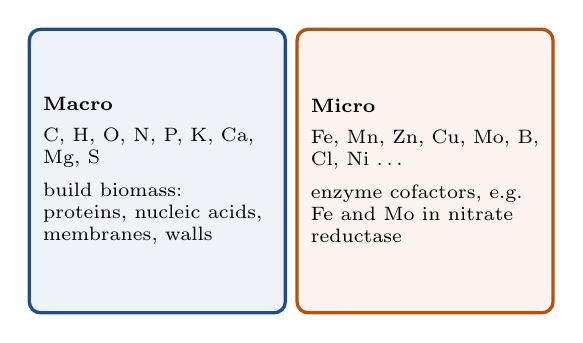
\begin{tikzpicture}[font=\scriptsize]
  \node[card=sea, text width=2.9cm, minimum height=3.6cm, anchor=north] at (-1.7,0) {\textbf{Macro}\\[3pt] C, H, O, N, P, K, Ca, Mg, S\\[4pt] build biomass: proteins, nucleic acids, membranes, walls};
  \node[card=warm, text width=2.9cm, minimum height=3.6cm, anchor=north] at (1.7,0) {\textbf{Micro}\\[3pt] Fe, Mn, Zn, Cu, Mo, B, Cl, Ni \ldots\\[4pt] enzyme cofactors, e.g.\ Fe and Mo in nitrate reductase};
\end{tikzpicture}
\fignote{Lists after Lobban and Harrison (1997, Table 5.2) and Hopkins and Hüner (2008, Table 4.4).}}
\end{frame}

% pos 11
\begin{frame}{About twenty elements are needed by algae}
\twocol{
\begin{itemize}
  \item Around 20 elements support critical metabolic pathways in algae
  \item Algae and land plants share most of them; amounts differ
  \item Some are needed only by certain groups (e.g.\ Si in diatoms)
\end{itemize}}{
\begin{tikzpicture}[font=\scriptsize]
  \foreach \e [count=\i from 0] in {C,H,O,N,P,K,Ca,Mg,S}
    \node[el=sea] at ({mod(\i,5)*1.0},{-floor(\i/5)*1.0}) {\e};
  \foreach \e [count=\i from 0] in {Fe,Mn,Zn,Cu,Mo,B,Cl,Co,Na,Br,I}
    \node[el=warm] at ({mod(\i,5)*1.0},{-2.4-floor(\i/5)*1.0}) {\e};
  \node[font=\scriptsize\bfseries, sea, anchor=west] at (-0.45,0.75) {macronutrients};
  \node[font=\scriptsize\bfseries, warm, anchor=west] at (-0.45,-1.65) {micronutrients and elements needed by some seaweeds};
\end{tikzpicture}
\fignote{See Lobban and Harrison (1997, Table 5.1) for the elements and their functions.}}
\end{frame}

% pos 12
\begin{frame}{Functions of essential elements in seaweeds}
\centering\scriptsize
\renewcommand{\arraystretch}{0.9}
\begin{tabular}{@{}>{\bfseries}l>{\raggedright\arraybackslash}p{5.9cm}>{\raggedright\arraybackslash}p{6.1cm}@{}}
Element & Probable functions & Examples of compounds\\\hline
N & major metabolic importance in compounds & amino acids, purines, pyrimidines, amino sugars, amines\\
P & structural, energy transfer & ATP, GTP, nucleic acids, phospholipids, coenzyme A\\
K & osmotic regulation, pH control, protein conformation & occurs mainly in ionic form\\
Ca & structural, enzyme activation, ion transport & calcium alginate, calcium carbonate\\
Mg & photosynthetic pigments, enzyme activation, ribosome stability & chlorophyll\\
S & active groups in enzymes and coenzymes, structural & cystine, glutathione, agar, carrageenan, sulfolipids\\
Fe & porphyrin molecules and enzymes & ferredoxin, cytochromes, nitrate reductase\\
Mn & electron transport in photosystem II & \\
Cu & electron transport in photosynthesis, enzymes & plastocyanin, amine oxidase\\
Zn & enzymes & carbonic anhydrase\\
Mo & nitrate reduction, ion absorption & nitrate reductase\\
Co & component of vitamin B$_{12}$ & B$_{12}$\\\hline
\end{tabular}
\fignote{After DeBoer (1981), in Lobban and Harrison (1997, Table 5.1). Selected rows.}
\end{frame}

% pos 13
\begin{frame}{Tissue concentrations in land plants}
\centering
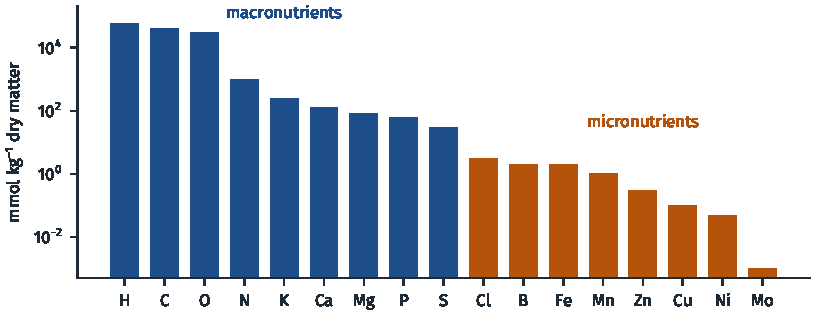
\includegraphics[width=0.86\textwidth]{fig_plant_tissue}
\fignote{Concentrations in dry matter considered adequate for normal growth of higher plants (Epstein 1972; Hopkins and Hüner 2008, Table 4.4). Logarithmic axis: macronutrients exceed micronutrients by several orders of magnitude.}
\end{frame}

% pos 14
\begin{frame}{Tissue and seawater concentrations}
\twocol{
\begin{itemize}
  \item C, H, O, N and P make up the bulk of algal dry matter
  \item Micronutrients and vitamins occur in much smaller amounts and rarely limit growth to the same extent
  \item N and P are about 100,000 times, and C about 10,000 times, more concentrated in the thallus than in seawater
  \item Much of tissue N is organic: compare the same dissolved form on both sides of the membrane
\end{itemize}}{
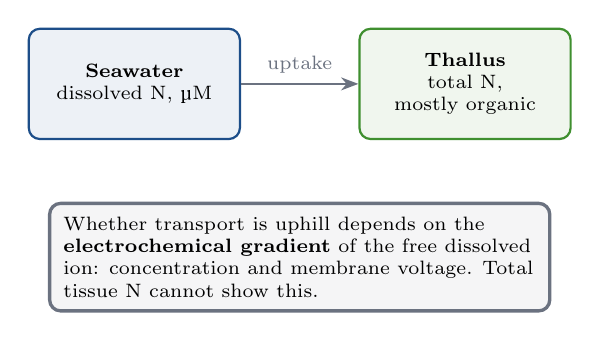
\begin{tikzpicture}[font=\scriptsize]
  \node[flow=sea, text width=2.4cm, minimum height=1.4cm] (w) at (-2.1,0) {\textbf{Seawater}\\ dissolved N, µM};
  \node[flow=leaf, text width=2.4cm, minimum height=1.4cm] (t) at (2.1,0) {\textbf{Thallus}\\ total N, mostly organic};
  \draw[arr] (w) -- node[above, font=\scriptsize] {uptake} (t);
  \node[card=grey, text width=6.0cm, font=\scriptsize] at (0,-2.2) {Whether transport is uphill depends on the \textbf{electrochemical gradient} of the free dissolved ion: concentration and membrane voltage. Total tissue N cannot show this.};
\end{tikzpicture}
\fignote{Concentration factors from Lobban and Harrison (1997, Table 5.2).}}
\end{frame}

% pos 15
\begin{frame}{Vitamins and organic nutrients}
\twocol{
\begin{itemize}
  \item Many algae also require \textbf{vitamins}: mainly B$_{12}$, thiamine and biotin
  \item These are often added to culture media to promote growth
  \item Some algae use \textbf{dissolved organic compounds}: amino acids as an N source, acetate as a C source
  \item Such mixotrophy is less common and is not the focus of this lecture
\end{itemize}}{
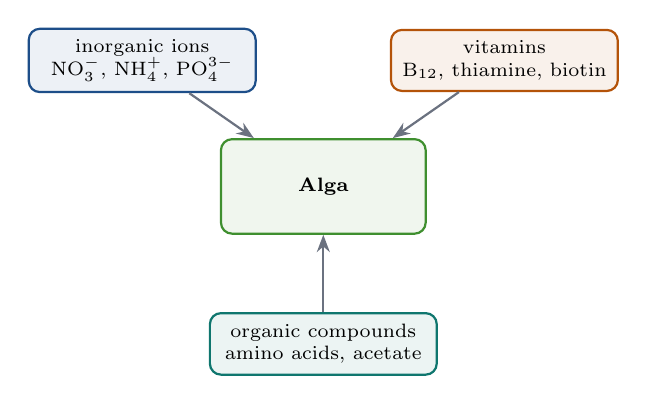
\begin{tikzpicture}[font=\scriptsize]
  \node[flow=leaf, minimum width=2.6cm, minimum height=1.2cm] (a) at (0,0) {\textbf{Alga}};
  \node[flow=sea, text width=2.6cm] (i) at (-2.3,1.6) {inorganic ions\\ NO$_3^-$, NH$_4^+$, PO$_4^{3-}$};
  \node[flow=warm, text width=2.6cm] (v) at (2.3,1.6) {vitamins\\ B$_{12}$, thiamine, biotin};
  \node[flow=accent, text width=2.6cm] (o) at (0,-2.0) {organic compounds\\ amino acids, acetate};
  \draw[arr] (i) -- (a); \draw[arr] (v) -- (a); \draw[arr] (o) -- (a);
\end{tikzpicture}
\fignote{Schematic.}}
\end{frame}

% pos 16
\begin{frame}{Elements are concentrated in seaweed tissue}
\twocol{
\begin{itemize}
  \item Ratio of mean concentration in seaweed dry matter to that in seawater
  \item N and P (red) are among the most concentrated macronutrients
  \item Trace metals such as Fe and Mn are scarce in seawater, so their ratios are very large
  \item Tissue values include organic and stored forms
\end{itemize}}{
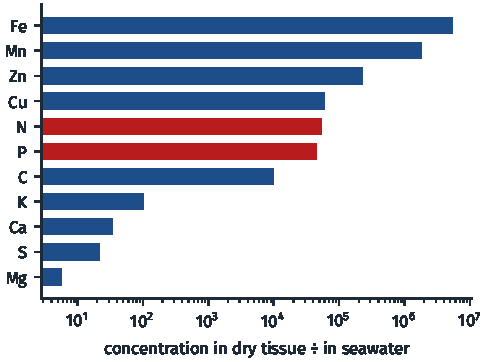
\includegraphics[width=\linewidth]{fig_concentration_factor}
\fignote{Calculated from DeBoer (1981), in Lobban and Harrison (1997, Table 5.2); logarithmic axis.}}
\end{frame}

% pos 17
\begin{frame}{Testing for a limiting nutrient}
\twocol{
\begin{itemize}
  \item Early work identified N as the nutrient most often limiting algal growth in the sea (Dugdale 1967)
  \item Adding N to seaweed aquaculture can greatly increase growth
  \item In some systems P limits, and P addition has similar effects
  \item Test with additions: control, +N, +P, +N+P, other conditions matched
  \item A null response to one nutrient leaves its role open: another factor may also restrict growth
\end{itemize}}{
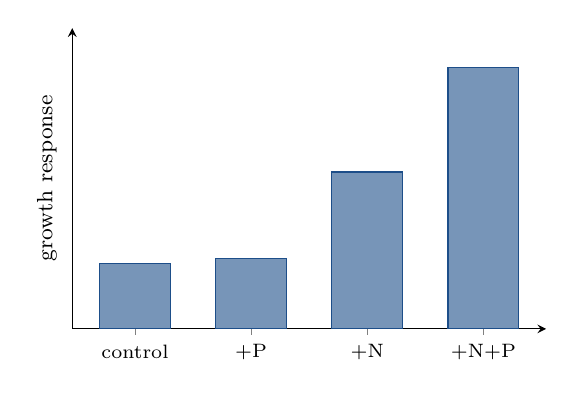
\begin{tikzpicture}[font=\scriptsize]
\begin{axis}[ybar, width=7.6cm, height=5.4cm, bar width=0.9cm, ymin=0, ymax=1.15,
  symbolic x coords={control,+P,+N,+N+P}, xtick=data, ytick=\empty, axis lines=left,
  ylabel={\footnotesize growth response}, x tick label style={font=\scriptsize}, enlarge x limits=0.18, clip=false]
  \addplot[fill=sea!60, draw=sea] coordinates {(control,0.25) (+P,0.27) (+N,0.6) (+N+P,1.0)};
\end{axis}
\end{tikzpicture}
\fignote{Schematic outcome for an alga primarily limited by N, with P limiting once N is added.}}
\end{frame}

% pos 18
\begin{frame}{The Redfield ratio}
\twocol{
\begin{itemize}
  \item Microalgae and seaweeds differ in the relative amounts of C, N and P
  \item Marine plankton: C:N:P about 106:16:1, the \textbf{Redfield ratio} (Redfield 1958)
  \item Benthic marine plants: about 550:30:1 (Atkinson and Smith 1983)
  \item Seaweeds hold much more C per P: structural carbon and storage polysaccharides
  \item These are empirical summaries; composition varies with species and conditions
\end{itemize}}{
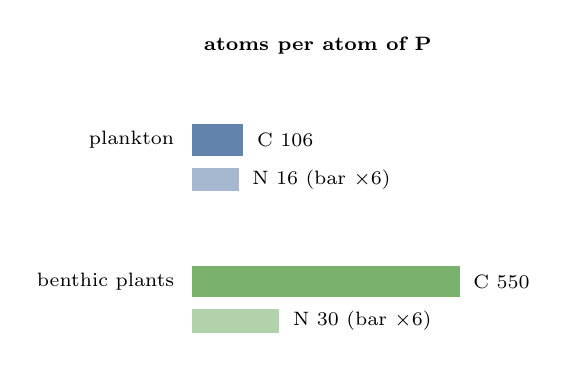
\begin{tikzpicture}[font=\scriptsize]
  \node[font=\scriptsize\bfseries] at (1.6,3.6) {atoms per atom of P};
  \foreach \lab/\c/\n/\y/\col in {plankton/106/16/2.4/sea, benthic plants/550/30/0.6/leaf}{
    \node[anchor=east, font=\scriptsize] at (-0.1,\y) {\lab};
    \fill[\col!70] (0,\y-0.2) rectangle ({\c/550*3.4},\y+0.2);
    \node[anchor=west, font=\scriptsize] at ({\c/550*3.4+0.05},\y) {C \c};
    \fill[\col!40] (0,\y-0.65) rectangle ({\n/550*3.4*6},\y-0.35);
    \node[anchor=west, font=\scriptsize] at ({\n/550*3.4*6+0.05},\y-0.5) {N \n\ (bar $\times$6)};
  }
\end{tikzpicture}
\fignote{N bars drawn six times longer than the C scale so that they remain visible.}}
\end{frame}

% pos 19
\begin{frame}{Which ratio answers which question?}
\twocol{
\begin{itemize}
  \item Reported optimal N:P ratios for seaweed cultivation vary widely (ca.\ 10:1 to 80:1)
  \item Ratios guide fertilising strategies in tank culture and predictions about eutrophication
  \item A deviation from a reference ratio suggests a hypothesis about nutrient status
  \item Test it with nutrient additions, tissue measurements and the growth response
\end{itemize}}{
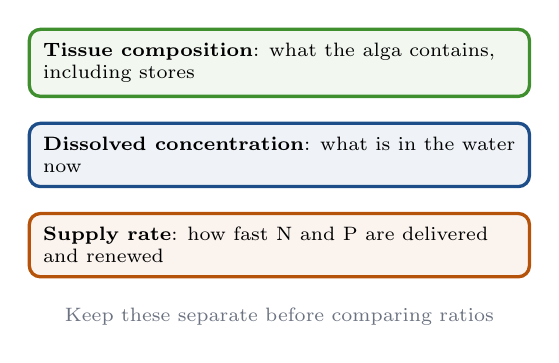
\begin{tikzpicture}[font=\scriptsize]
  \node[card=leaf, text width=6.0cm] (a) {\textbf{Tissue composition}: what the alga contains, including stores};
  \node[card=sea, text width=6.0cm, below=0.3cm of a] (b) {\textbf{Dissolved concentration}: what is in the water now};
  \node[card=warm, text width=6.0cm, below=0.3cm of b] (c) {\textbf{Supply rate}: how fast N and P are delivered and renewed};
  \node[font=\scriptsize, grey, below=0.25cm of c, text width=6cm, align=center] {Keep these separate before comparing ratios};
\end{tikzpicture}}
\end{frame}

% pos 20
\begin{frame}{Liebig's law of the minimum}
\twocol{
\begin{itemize}
  \item Justus von Liebig (1803--1873) studied the chemistry of fertilisers
  \item If one essential nutrient is deficient, growth is poor even when all others are plentiful
  \item Supplying the deficient element increases growth until it no longer limits
  \item Beyond that point another resource is in shortest supply and limits instead
\end{itemize}}{
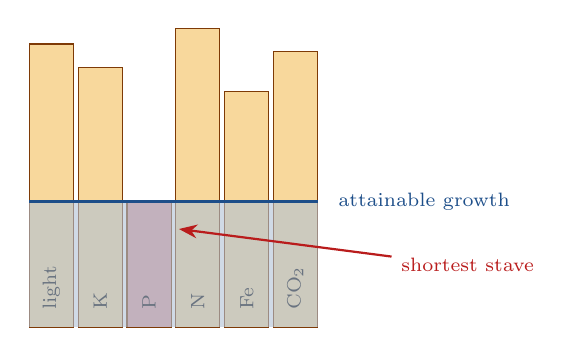
\begin{tikzpicture}[font=\scriptsize]
  \foreach \lab/\hh/\c [count=\i from 0] in {light/3.6/sand!55, K/3.3/sand!55, P/1.6/hot!45, N/3.8/sand!55, Fe/3.0/sand!55, CO$_2$/3.5/sand!55}{
    \fill[\c, draw=warm!70!black] (\i*0.62,0) rectangle (\i*0.62+0.56,\hh);
    \node[rotate=90, anchor=west] at (\i*0.62+0.28,0.1) {\lab};
  }
  \fill[sea!35, opacity=0.6] (0,0) rectangle (3.66,1.6);
  \draw[sea, very thick] (0,1.6) -- (3.66,1.6);
  \node[sea, anchor=west, font=\scriptsize] at (3.8,1.6) {attainable growth};
  \draw[-{Stealth}, hot, thick] (4.6,0.9) -- (1.9,1.25);
  \node[hot, anchor=west, font=\scriptsize] at (4.6,0.8) {shortest stave};
\end{tikzpicture}
\fignote{Schematic: the stave barrel. Water rises only to the shortest stave.}}
\end{frame}

% pos 21
\begin{frame}{Limitation reflects requirement and supply}
\twocol{
\begin{itemize}
  \item Ambient concentration reflects the balance between the alga's requirement and the rate of supply
  \item Physical conditions and traits of the alga also restrict growth
  \item Several factors can restrict growth at once, or one after another
\end{itemize}}{
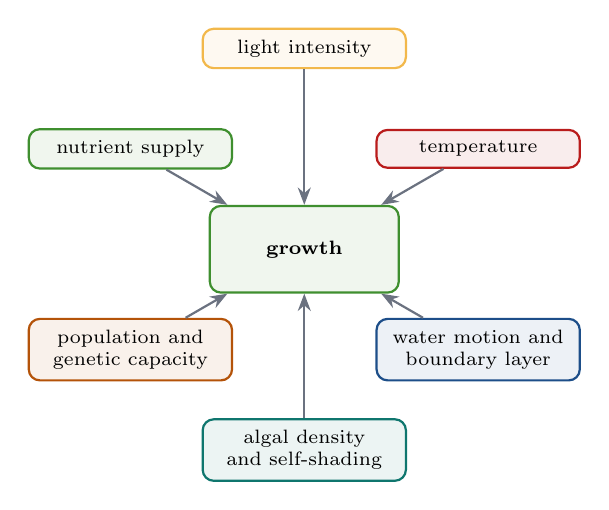
\begin{tikzpicture}[font=\scriptsize]
  \node[flow=leaf, minimum width=2.4cm, minimum height=1.1cm] (g) at (0,0) {\textbf{growth}};
  \foreach \t/\a/\c in {light intensity/90/sand, temperature/30/hot, water motion and boundary layer/-30/sea, algal density and self-shading/-90/accent, population and genetic capacity/-150/warm, nutrient supply/150/leaf}{
    \node[flow=\c, text width=2.3cm, font=\scriptsize] (n\a) at (\a:2.55) {\t};
    \draw[arr] (n\a) -- (g);
  }
\end{tikzpicture}
\fignote{Schematic.}}
\end{frame}

% pos 22
\begin{frame}{Accounting with the minimum model}
\twocol{
\begin{itemize}
  \item Suppose each new biomass unit needs 10 µmol N and 1 µmol P
  \item With 20 µmol N and 1 µmol P: P permits one unit; 10 µmol N remain unused
  \item Add 1 µmol P: the same N supports two units
  \item Beyond 2 µmol P, N limits
  \item Illustrative requirements, not a universal seaweed ratio
\end{itemize}}{
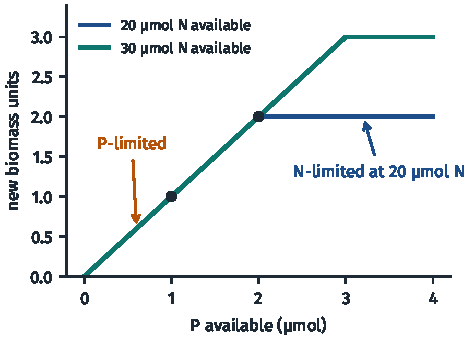
\includegraphics[width=\linewidth]{fig_liebig}
\fignote{Attainable biomass = min(N/10, P/1). Real responses involve reserves, variable composition and other constraints.}}
\end{frame}

% pos 23
\begin{frame}{Luxury consumption}
\twocol{
\begin{itemize}
  \item Uptake of more N or P than growth needs at the time
  \item The excess may remain in the medium, be stored as inorganic N or P in vacuoles, or be assimilated into organic compounds
  \item Stores are mobilised for growth when external supply declines
  \item An advantage where supply fluctuates; also used as a fertilising strategy in aquaculture
\end{itemize}}{
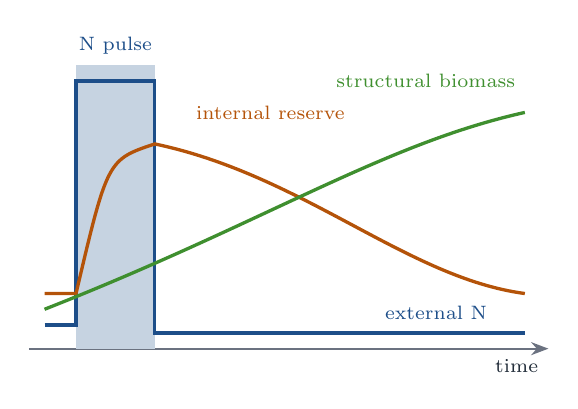
\begin{tikzpicture}[font=\scriptsize]
  \draw[arr] (0,0) -- (6.6,0) node[below left, ink] {time};
  \fill[sea!25] (0.6,0) rectangle (1.6,3.6);
  \node[sea, font=\scriptsize] at (1.1,3.85) {N pulse};
  \draw[very thick, sea] (0.2,0.3) -- (0.6,0.3) -- (0.6,3.4) -- (1.6,3.4) -- (1.6,0.2) -- (6.3,0.2);
  \draw[very thick, warm] (0.2,0.7) -- (0.6,0.7) .. controls (1.0,2.4) .. (1.6,2.6) .. controls (3.5,2.2) and (4.8,0.9) .. (6.3,0.7);
  \draw[very thick, leaf] (0.2,0.5) .. controls (3,1.6) and (4.5,2.6) .. (6.3,3.0);
  \node[sea, anchor=west, font=\scriptsize] at (4.4,0.45) {external N};
  \node[warm, anchor=west, font=\scriptsize] at (2.0,3.0) {internal reserve};
  \node[leaf, anchor=east, font=\scriptsize] at (6.3,3.4) {structural biomass};
\end{tikzpicture}
\fignote{Schematic. Uptake and growth occur at different times; storage capacity varies among species, tissues and conditions.}}
\end{frame}

% pos 24
\begin{frame}{Nitrogen as the worked example}
\twocol{
\begin{itemize}
  \item N most often limits algal growth in the sea
  \item N pollution drives eutrophication
  \item Uptake and assimilation of other nutrients follow similar principles
  \item Most concepts apply to both macroalgae and microalgae
\end{itemize}}{
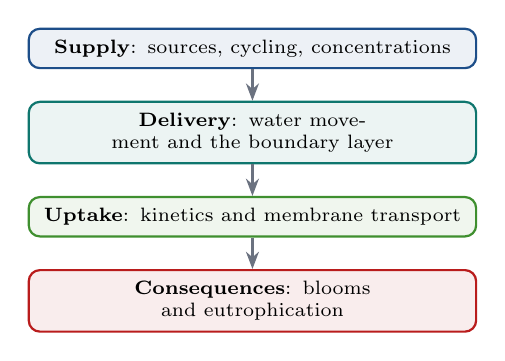
\begin{tikzpicture}[font=\scriptsize]
  \node[flow=sea, text width=5.4cm] (a) {\textbf{Supply}: sources, cycling, concentrations};
  \node[flow=accent, text width=5.4cm, below=0.4cm of a] (b) {\textbf{Delivery}: water movement and the boundary layer};
  \node[flow=leaf, text width=5.4cm, below=0.4cm of b] (c) {\textbf{Uptake}: kinetics and membrane transport};
  \node[flow=hot, text width=5.4cm, below=0.4cm of c] (d) {\textbf{Consequences}: blooms and eutrophication};
  \draw[arr] (a) -- (b); \draw[arr] (b) -- (c); \draw[arr] (c) -- (d);
\end{tikzpicture}
\fignote{The route this lecture follows.}}
\end{frame}

% pos 26
\begin{frame}{Sources of nitrogen in the sea}
\twocol{
\begin{itemize}
  \item N$_2$ gas: about 78\% of the atmosphere; dissolved N$_2$ remains N$_2$ until fixed
  \item Biological N fixation converts N$_2$ to forms available to the food web
  \item Rivers, wastewater and atmospheric deposition bring reactive N to coastal waters
  \item Recycling within the ocean is of major importance
  \item Upwelling moves existing nutrient-rich water upwards
\end{itemize}}{
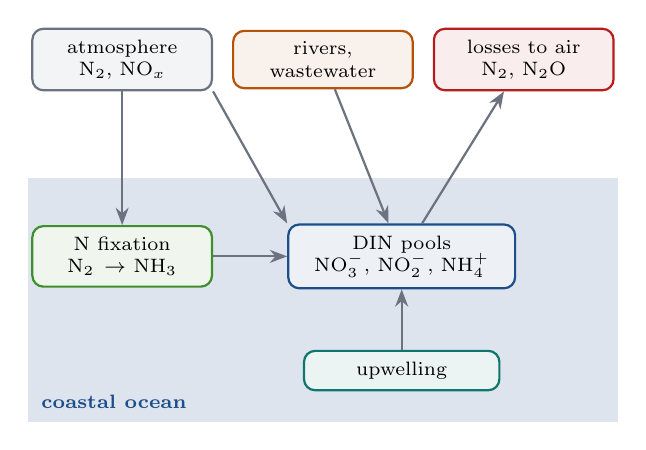
\begin{tikzpicture}[font=\scriptsize]
  \fill[sea!15] (-3.75,-2.6) rectangle (3.75,0.5);
  \node[sea, font=\scriptsize\bfseries, anchor=south west] at (-3.7,-2.55) {coastal ocean};
  \node[flow=grey, text width=2.0cm] (atm) at (-2.55,2.0) {atmosphere\\ N$_2$, NO$_x$};
  \node[flow=warm, text width=2.0cm] (riv) at (0,2.0) {rivers,\\ wastewater};
  \node[flow=hot, text width=2.0cm] (out) at (2.55,2.0) {losses to air\\ N$_2$, N$_2$O};
  \node[flow=leaf, text width=2.0cm] (fix) at (-2.55,-0.5) {N fixation\\ N$_2\rightarrow$ NH$_3$};
  \node[flow=sea, text width=2.6cm] (din) at (1.0,-0.5) {DIN pools\\ NO$_3^-$, NO$_2^-$, NH$_4^+$};
  \node[flow=accent, text width=2.2cm] (up) at (1.0,-1.95) {upwelling};
  \draw[arr] (atm) -- (fix); \draw[arr] (atm.south east) -- (din.north west);
  \draw[arr] (riv) -- (din); \draw[arr] (din) -- (out);
  \draw[arr] (fix) -- (din); \draw[arr] (up) -- (din);
\end{tikzpicture}
\fignote{Schematic. Pool sizes vary with depth, oxygen, biological activity and place.}}
\end{frame}

% pos 27
\begin{frame}{Fixation and transformations of nitrogen}
\twocol{
\begin{itemize}
  \item N-fixing microorganisms, including some cyanobacteria, reduce N$_2$ to ammonia
  \item Most photoautotrophs use nitrate, nitrite and ammonium
  \item \textbf{DIN} = NO$_3^-$ + NO$_2^-$ + NH$_4^+$, as N; it excludes dissolved N$_2$
  \item Nitrite is an intermediate; it accumulates where production exceeds consumption
\end{itemize}}{
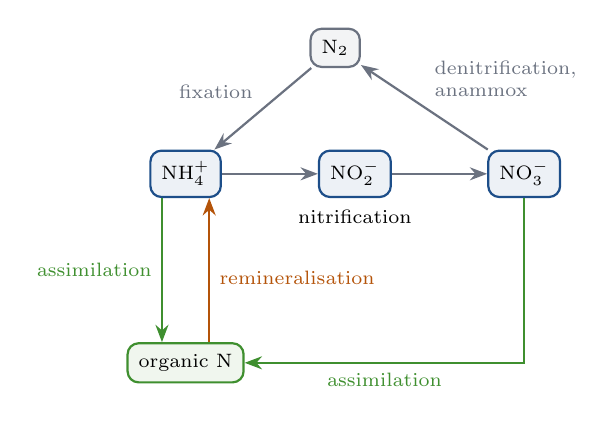
\begin{tikzpicture}[font=\scriptsize, node distance=1.0cm]
  \node[flow=grey] (n2) at (0,2.4) {N$_2$};
  \node[flow=sea] (nh4) at (-1.9,0.8) {NH$_4^+$};
  \node[flow=sea] (no2) at (0.25,0.8) {NO$_2^-$};
  \node[flow=sea] (no3) at (2.4,0.8) {NO$_3^-$};
  \node[flow=leaf] (org) at (-1.9,-1.6) {organic N};
  \draw[arr] (n2) -- node[above left, font=\scriptsize] {fixation} (nh4);
  \draw[arr] (nh4) -- (no2); \draw[arr] (no2) -- (no3);
  \node[font=\scriptsize] at (0.25,0.25) {nitrification};
  \draw[arr] (no3) -- node[above right, font=\scriptsize, align=left] {denitrification,\\ anammox} (n2);
  \draw[arr, leaf] ([xshift=-3mm]nh4.south) -- node[left, font=\scriptsize] {assimilation} ([xshift=-3mm]org.north);
  \draw[arr, warm] ([xshift=3mm]org.north) -- node[right, font=\scriptsize, pos=0.45] {remineralisation} ([xshift=3mm]nh4.south);
  \draw[arr, leaf] (no3.south) |- node[pos=0.75, below, font=\scriptsize] {assimilation} (org.east);
\end{tikzpicture}
\fignote{Schematic.}}
\end{frame}

% pos 29
\begin{frame}{Terms for the pools of N and P}
\twocol{
\begin{itemize}
  \item Pools are defined by chemical form and by whether they pass through a filter
  \item The same terms apply on land, where most transformations happen in soil and leaf litter
\end{itemize}}{
\centering\footnotesize
\renewcommand{\arraystretch}{1.4}
\begin{tabular}{@{}>{\bfseries\color{sea}}l>{\raggedright\arraybackslash}p{5.0cm}@{}}
DIN & dissolved inorganic N: NO$_3^-$, NO$_2^-$, NH$_4^+$\\
DIP & dissolved inorganic P: phosphate\\
DON & dissolved organic N: e.g.\ urea, amino acids\\
DOP & dissolved organic P\\
POM & particulate organic matter, with its N and P\\\hline
\end{tabular}}
\end{frame}

% pos 30
\begin{frame}{Units of nutrient concentration}
\twocol{
\begin{itemize}
  \item Concentrations are usually given in µM (µmol L$^{-1}$)
  \item Older literature uses microgram atoms per litre (µg-at L$^{-1}$)
  \item For a single element, µg-at L$^{-1}$ equals µM numerically
  \item Exercise: complete the table
\end{itemize}}{
\centering\footnotesize
\renewcommand{\arraystretch}{1.35}
\begin{tabular}{cc}
\textbf{NH$_4^+$ and NO$_3^-$ (µmol L$^{-1}$)} & \textbf{(µg-at L$^{-1}$)}\\\hline
2 & ?\\ 3 & ?\\ 12 & ?\\ 21 & ?\\ 30 & ?\\\hline
\end{tabular}
\fignote{Exercise.}}
\end{frame}

% pos 31
\begin{frame}{From µmol to µg of nitrogen}
\twocol{
\begin{itemize}
  \item Molecular (atomic) mass, MM, in g mol$^{-1}$
  \item For N, MM = 14.0067 g mol$^{-1}$, equivalently µg µmol$^{-1}$
  \item Calculations for N and P use the mass of the element only, not the whole ion
\end{itemize}}{
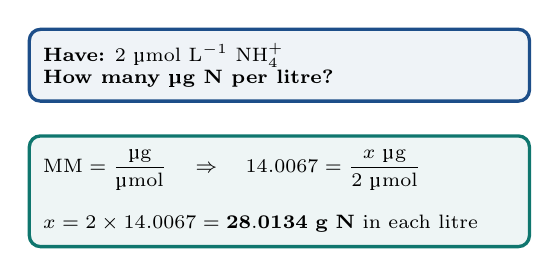
\begin{tikzpicture}[font=\scriptsize]
  \node[card=sea, text width=6.0cm] (q) {\textbf{Have:} 2 µmol L$^{-1}$ NH$_4^+$\\ \textbf{How many µg N per litre?}};
  \node[card=accent, text width=6.0cm, below=0.4cm of q] (w) {
    $\displaystyle \text{MM} = \frac{\text{µg}}{\text{µmol}} \quad\Rightarrow\quad 14.0067 = \frac{x\ \text{µg}}{2\ \text{µmol}}$\\[8pt]
    $x = 2 \times 14.0067 = \mathbf{28.0134\ µg\ N}$ in each litre};
\end{tikzpicture}}
\end{frame}

% pos 32
\begin{frame}{SI prefixes}
\twocol{
\begin{itemize}
  \item Know the prefixes and the powers of ten they stand for
  \item In nutrient work you will meet g, mg, µg, ng and pg; mol, mmol, µmol and nmol; L and mL
  \item Each step in this range is a factor of 1,000
\end{itemize}}{
\centering\footnotesize
\renewcommand{\arraystretch}{1.05}
\begin{tabular}{@{}llr@{\hspace{1.0em}}llr@{}}
\textbf{Prefix} & \textbf{Symbol} & & \textbf{Prefix} & \textbf{Symbol} & \\\hline
exa & E & $10^{18}$ & deci & d & $10^{-1}$\\
peta & P & $10^{15}$ & centi & c & $10^{-2}$\\
tera & T & $10^{12}$ & milli & m & $10^{-3}$\\
giga & G & $10^{9}$ & micro & µ & $10^{-6}$\\
mega & M & $10^{6}$ & nano & n & $10^{-9}$\\
kilo & k & $10^{3}$ & pico & p & $10^{-12}$\\
hecto & h & $10^{2}$ & femto & f & $10^{-15}$\\
deka & da & $10^{1}$ & atto & a & $10^{-18}$\\\hline
\end{tabular}}
\end{frame}

% pos 33
\begin{frame}{Nitrogen concentrations in the ocean}
\twocol{
\begin{itemize}
  \item State the N form, depth and units
  \item Some tropical and temperate coastal seas (e.g.\ temperate Australia): almost immeasurable all year
  \item Coastal upwelling (California, Benguela, Canary, Humboldt currents): seasonal peaks
  \item Upwelled N arrives in pulses every week or two, each lasting one to several days
  \item Saldanha Bay: nitrate from undetectable to around 30--40 µM (Smit 2002)
\end{itemize}}{
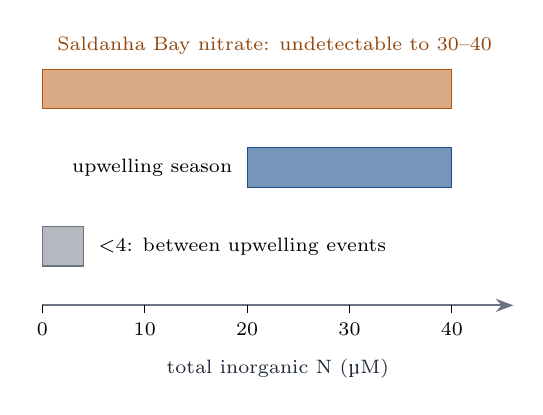
\begin{tikzpicture}[font=\scriptsize, x=0.13cm]
  \draw[arr] (0,0) -- (46,0);
  \node[ink] at (23,-0.8) {total inorganic N (µM)};
  \foreach \v in {0,10,20,30,40} {\draw (\v,0) -- (\v,-0.1) node[below, font=\scriptsize] {\v};}
  \fill[grey!50, draw=grey] (0,0.5) rectangle (4,1.0);
  \node[anchor=west, font=\scriptsize] at (4.5,0.75) {$<$4: between upwelling events};
  \fill[sea!60, draw=sea] (20,1.5) rectangle (40,2.0);
  \node[anchor=east, font=\scriptsize] at (19.5,1.75) {upwelling season};
  \fill[warm!50, draw=warm] (0,2.5) rectangle (40,3.0);
  \node[anchor=west, font=\scriptsize, warm!80!black] at (0.5,3.3) {Saldanha Bay nitrate: undetectable to 30--40};
\end{tikzpicture}
\fignote{Upwelling systems; inorganic P is ca.\ 2 µM in season and $<$0.2 µM otherwise. Exercise: 40 µM N $\div$ 2 µM P gives a molar N:P of 20:1.}}
\end{frame}

% pos 34
\begin{frame}{Oligotrophic, mesotrophic, eutrophic}
\twocol{
\begin{itemize}
  \item Broadly low, intermediate and high nutrient availability or productivity
  \item State the indicator and the context
  \item Low dissolved nutrients can also mean active uptake, with high production
  \item Upwelling regions can be highly productive
  \item Eutrophic conditions may be natural or caused by people
\end{itemize}}{
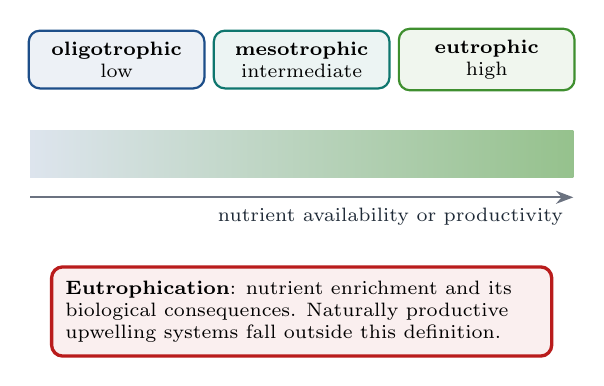
\begin{tikzpicture}[font=\scriptsize]
  \shade[left color=sea!15, right color=leaf!55] (-3.45,0) rectangle (3.45,0.6);
  \draw[arr] (-3.45,-0.25) -- (3.45,-0.25) node[below left, font=\scriptsize, ink] {nutrient availability or productivity};
  \node[flow=sea, text width=1.95cm, font=\scriptsize] at (-2.35,1.5) {\textbf{oligotrophic}\\ low};
  \node[flow=accent, text width=1.95cm, font=\scriptsize] at (0,1.5) {\textbf{mesotrophic}\\ intermediate};
  \node[flow=leaf, text width=1.95cm, font=\scriptsize] at (2.35,1.5) {\textbf{eutrophic}\\ high};
  \node[card=hot, text width=6.0cm, font=\scriptsize] at (0,-1.7) {\textbf{Eutrophication}: nutrient enrichment and its biological consequences. Naturally productive upwelling systems fall outside this definition.};
\end{tikzpicture}}
\end{frame}

% pos 35
\begin{frame}{A problem of global proportions}
\twocol{
\begin{itemize}
  \item N limitation is seldom the problem (except in aquaculture)
  \item The Haber--Bosch process short-circuited the N cycle
  \item More N is now fixed each year by human activity than by natural terrestrial fixation (Gruber and Galloway 2008)
  \item First benefit: higher crop production; later costs in fresh, coastal and marine waters
  \item Eutrophication is the oldest water-quality problem of lakes and coasts
\end{itemize}}{
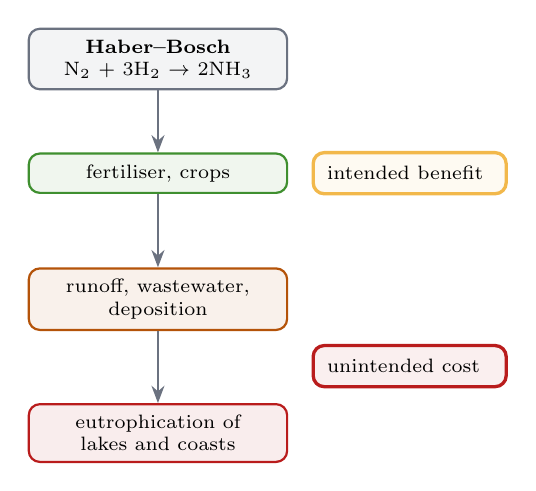
\begin{tikzpicture}[font=\scriptsize]
  \node[flow=grey, text width=3.0cm] (hb) at (0,2.9) {\textbf{Haber--Bosch}\\ N$_2$ + 3H$_2$ $\rightarrow$ 2NH$_3$};
  \node[flow=leaf, text width=3.0cm] (f) at (0,1.45) {fertiliser, crops};
  \node[flow=warm, text width=3.0cm] (r) at (0,-0.15) {runoff, wastewater,\\ deposition};
  \node[flow=hot, text width=3.0cm] (e) at (0,-1.85) {eutrophication of\\ lakes and coasts};
  \draw[arr] (hb) -- (f); \draw[arr] (f) -- (r); \draw[arr] (r) -- (e);
  \node[card=sand, text width=2.1cm, font=\scriptsize, anchor=west] at (1.95,1.45) {intended benefit};
  \node[card=hot, text width=2.1cm, font=\scriptsize, anchor=west] at (1.95,-1.0) {unintended cost};
\end{tikzpicture}
\fignote{Self-study: Fisher and Fisher (2001), \textit{The nitrogen bomb}.}}
\end{frame}

% pos 37
\begin{frame}{Eutrophication}
\twocol{
\begin{itemize}
  \item Enrichment can cause blooms of opportunistic macroalgae such as \textit{Ulva} (incl.\ former \textit{Enteromorpha}) and \textit{Cladophora}, and of phytoplankton
  \item Effects include shifts in community composition: diversity, abundance and biomass
  \item In severe cases, decomposition of bloom biomass causes anoxia
  \item The response depends on the receiving system and the scale of the inputs
\end{itemize}}{
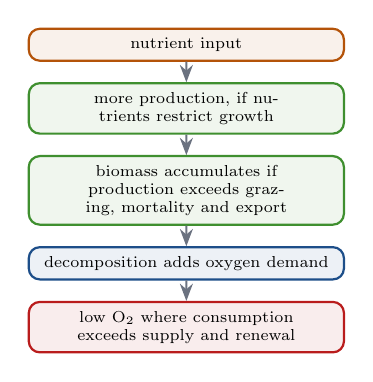
\begin{tikzpicture}[font=\scriptsize, node distance=0.32cm, scale=0.82, transform shape]
  \node[flow=warm, text width=4.6cm] (a) {nutrient input};
  \node[flow=leaf, text width=4.6cm, below=of a] (b) {more production, if nutrients restrict growth};
  \node[flow=leaf, text width=4.6cm, below=of b] (c) {biomass accumulates if production exceeds grazing, mortality and export};
  \node[flow=sea, text width=4.6cm, below=of c] (d) {decomposition adds oxygen demand};
  \node[flow=hot, text width=4.6cm, below=of d] (e) {low O$_2$ where consumption exceeds supply and renewal};
  \draw[arr] (a) -- (b); \draw[arr] (b) -- (c); \draw[arr] (c) -- (d); \draw[arr] (d) -- (e);
\end{tikzpicture}
\fignote{Schematic. Each step has conditions; none follows inevitably.}}
\end{frame}

% pos 38
\begin{frame}{Blooms: nutrients and form}
\twocol{
\begin{itemize}
  \item Bloom development depends on the extra nutrient pool and on the morphology and physiology of the alga
  \item Functional form model (Littler and Littler 1980)
  \item High SA:V forms, such as sheet-like \textit{Ulva} and finely branched \textit{Cladophora}, take up nutrients faster than coarse, thick thalli (Wallentinus 1984)
  \item Faster uptake can give an advantage under eutrophic conditions (Rosenberg and Ramus 1984)
\end{itemize}}{
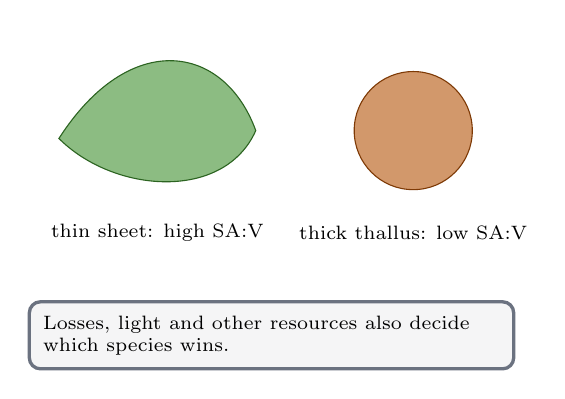
\begin{tikzpicture}[font=\scriptsize]
  \fill[leaf!60, draw=leaf!70!black] (-2.9,0.2) .. controls (-2.0,1.6) and (-0.8,1.4) .. (-0.4,0.3) .. controls (-0.8,-0.6) and (-2.2,-0.5) .. cycle;
  \node at (-1.65,-1.0) {thin sheet: high SA:V};
  \fill[warm!60, draw=warm!70!black] (1.6,0.3) circle (0.75);
  \node at (1.6,-1.0) {thick thallus: low SA:V};
  \node[card=grey, text width=5.8cm, font=\scriptsize] at (-0.2,-2.3) {Losses, light and other resources also decide which species wins.};
\end{tikzpicture}
\fignote{Schematic.}}
\end{frame}

% pos 39
\begin{frame}{Surface area to volume ratio and uptake}
\twocol{
\begin{itemize}
  \item Why do only some species respond to nutrient additions?
  \item How do others persist, or thrive, in oligotrophic or mesotrophic water?
  \item At the same flux per unit active surface, more area per gram gives more uptake per gram
  \item Water renewal and tissue condition change this comparison
\end{itemize}}{
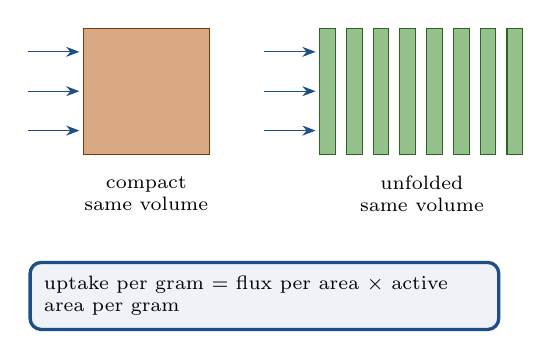
\begin{tikzpicture}[font=\scriptsize]
  \fill[warm!50, draw=warm!70!black] (-2.6,0) rectangle (-1.0,1.6);
  \node[align=center] at (-1.8,-0.5) {compact\\ same volume};
  \foreach \i in {0,...,7} \fill[leaf!55, draw=leaf!70!black] (0.4+\i*0.34,0) rectangle (0.6+\i*0.34,1.6);
  \node[align=center] at (1.7,-0.5) {unfolded\\ same volume};
  \foreach \y in {0.3,0.8,1.3} {\draw[-{Stealth}, sea] (-3.3,\y) -- (-2.65,\y); \draw[-{Stealth}, sea] (-0.3,\y) -- (0.35,\y);}
  \node[card=sea, text width=5.6cm, font=\scriptsize] at (-0.3,-1.8) {uptake per gram = flux per area $\times$ active area per gram};
\end{tikzpicture}
\fignote{Schematic; see concept 6 in Lecture 9c.}}
\end{frame}

% pos 40
\begin{frame}{The route of DIN into the cell}
\begin{center}
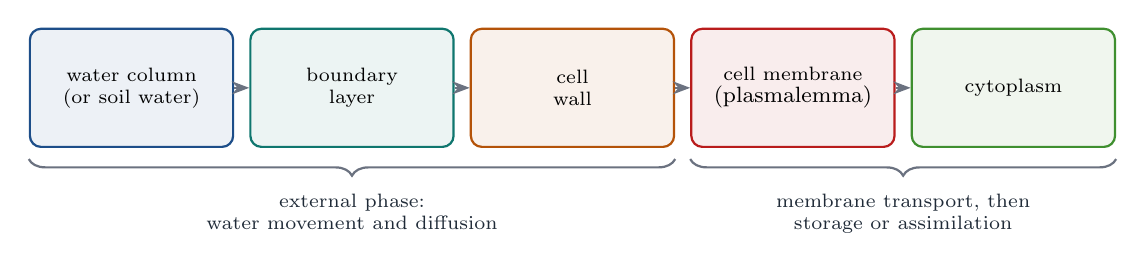
\begin{tikzpicture}[font=\scriptsize]
  \foreach \t/\c/\x [count=\k] in {{water column\\ (or soil water)}/sea/0, {boundary\\ layer}/accent/2.8, {cell\\ wall}/warm/5.6, {cell membrane\\ {\footnotesize (plasmalemma)}}/hot/8.4, cytoplasm/leaf/11.2}
    \node[flow=\c, text width=2.3cm, minimum height=1.5cm] (n\k) at (\x,0) {\t};
  \foreach \a/\b in {1/2, 2/3, 3/4, 4/5} \draw[arr] (n\a) -- (n\b);
  \draw[decorate, decoration={brace, amplitude=6pt, mirror}, thick, grey] ([yshift=-4pt]n1.south west) -- ([yshift=-4pt]n3.south east) node[midway, below=9pt, font=\scriptsize, ink, align=center] {external phase:\\ water movement and diffusion};
  \draw[decorate, decoration={brace, amplitude=6pt, mirror}, thick, grey] ([yshift=-4pt]n4.south west) -- ([yshift=-4pt]n5.south east) node[midway, below=9pt, font=\scriptsize, ink, align=center] {membrane transport, then\\ storage or assimilation};
\end{tikzpicture}
\end{center}
\fignote{Either phase can restrict nutrient acquisition.}
\end{frame}

% pos 41
\begin{frame}{Uptake is a two-stage process}
\twocol{
\begin{itemize}
  \item (i) Diffusion across the boundary layer next to the thallus
  \item (ii) Transport across the membrane and processing inside the alga
  \item When delivery is fast, membrane transport or processing sets the rate
  \item When kinetic capacity outruns delivery, uptake is limited by diffusion
\end{itemize}}{
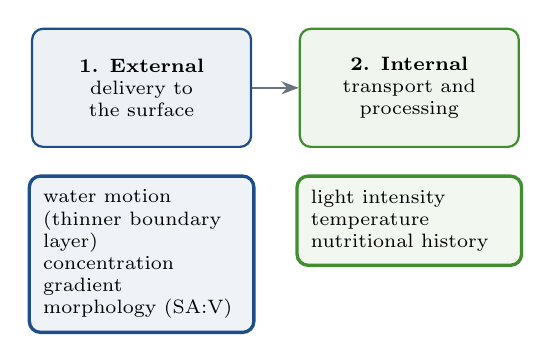
\begin{tikzpicture}[font=\scriptsize]
  \node[flow=sea, text width=2.5cm, minimum height=1.5cm] (e) at (-1.7,0) {\textbf{1. External}\\ delivery to the surface};
  \node[flow=leaf, text width=2.5cm, minimum height=1.5cm] (i) at (1.7,0) {\textbf{2. Internal}\\ transport and processing};
  \draw[arr] (e) -- (i);
  \node[card=sea, text width=2.5cm, font=\scriptsize, anchor=north] at (-1.7,-1.1) {water motion (thinner boundary layer)\\ concentration gradient\\ morphology (SA:V)};
  \node[card=leaf, text width=2.5cm, font=\scriptsize, anchor=north] at (1.7,-1.1) {light intensity\\ temperature\\ nutritional history};
\end{tikzpicture}
\fignote{The two stages are coupled.}}
\end{frame}

% pos 42
\begin{frame}{Boundary layer thickness and water movement}
\twocol{
\begin{itemize}
  \item Uptake depletes the water at the surface: a \textbf{concentration boundary layer}
  \item Flux across a layer of effective thickness $\delta$:
  \[J_{\text{in}} \approx D\,\frac{C_b - C_s}{\delta}\]
  \item Faster flow thins the layer and shortens the diffusion distance
  \item Stirring changes delivery and the concentration field; $D$ stays the same at a given temperature
\end{itemize}}{
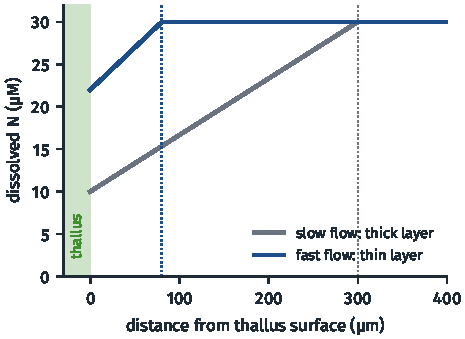
\includegraphics[width=\linewidth]{fig_bl_flow}
\fignote{Schematic profiles at the same uptake flux; $C_b$ bulk and $C_s$ surface concentration.}}
\end{frame}

% pos 43
\begin{frame}{Concentration gradient and diffusive supply}
\twocol{
\begin{itemize}
  \item High bulk [DIN]: large gradient, fast diffusive supply
  \item Low bulk [DIN]: small gradient, slow supply
  \item $C_s$ results from the balance of delivery and uptake
  \item In slow water, higher external concentration partly offsets a thick boundary layer
\end{itemize}}{
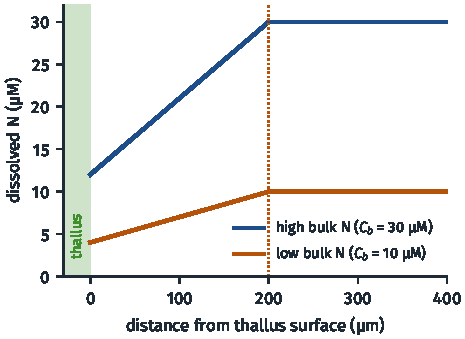
\includegraphics[width=\linewidth]{fig_bl_conc}
\fignote{Schematic profiles for the same layer thickness.}}
\end{frame}

% pos 44
\begin{frame}{Nutritional history}
\twocol{
\begin{itemize}
  \item Growth during low external N draws down internal reserves
  \item N-starved tissue may show fast \textit{initial} uptake after a pulse
  \item N-replete tissue takes up more slowly
  \item Possible causes: internal feedback, demand, changes in uptake machinery
  \item Depends on prior conditions and tissue health; the effect of starvation length varies
\end{itemize}}{
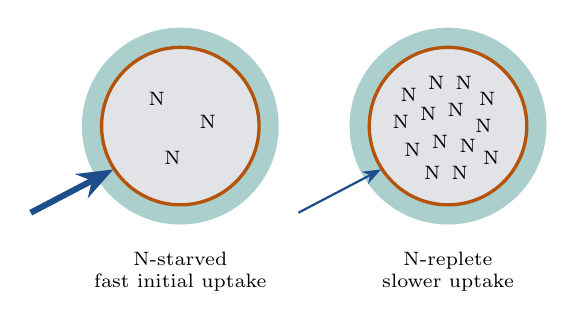
\begin{tikzpicture}[font=\scriptsize]
  \foreach \x/\lab/\w/\pts in {-1.7/{N-starved\\ fast initial uptake}/2.2/{(-0.3,0.35),(0.35,0.05),(-0.1,-0.4)}, 1.7/{N-replete\\ slower uptake}/0.8/{(-0.5,0.4),(-0.15,0.55),(0.2,0.55),(0.5,0.35),(-0.6,0.05),(-0.25,0.15),(0.1,0.2),(0.45,0.0),(-0.45,-0.3),(-0.1,-0.2),(0.25,-0.25),(0.55,-0.4),(-0.2,-0.6),(0.15,-0.6)}}{
    \fill[accent!35] (\x,0) circle (1.25);
    \fill[grey!20, draw=warm, very thick] (\x,0) circle (1.0);
    \begin{scope}[shift={(\x,0)}] \foreach \q in \pts {\node[font=\scriptsize] at \q {N};} \end{scope}
    \draw[-{Stealth}, sea, line width=\w pt] ($(\x,0)+(-1.9,-1.1)$) -- ($(\x,0)+(-0.85,-0.55)$);
    \node[align=center] at (\x,-1.85) {\lab};
  }
\end{tikzpicture}
\fignote{Schematic. Arrow width: relative uptake rate.}}
\end{frame}

% pos 45
\begin{frame}{Measuring uptake kinetics}
\twocol{
\begin{itemize}
  \item Uptake can be measured \textit{in situ} or under controlled laboratory conditions
  \item Usually from the \textbf{disappearance} of nutrient from the medium over a time interval after adding the alga
  \item Two designs: multiple flask (batch) and perturbation
  \item Depletion data give uptake rates, and from these the uptake kinetics
\end{itemize}}{
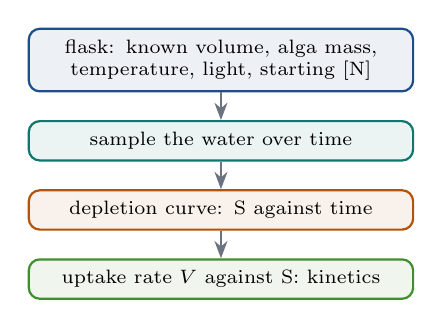
\begin{tikzpicture}[font=\scriptsize]
  \node[flow=sea, text width=4.6cm] (a) {flask: known volume, alga mass, temperature, light, starting [N]};
  \node[flow=accent, text width=4.6cm, below=0.35cm of a] (b) {sample the water over time};
  \node[flow=warm, text width=4.6cm, below=0.35cm of b] (c) {depletion curve: S against time};
  \node[flow=leaf, text width=4.6cm, below=0.35cm of c] (d) {uptake rate $V$ against S: kinetics};
  \draw[arr] (a) -- (b); \draw[arr] (b) -- (c); \draw[arr] (c) -- (d);
\end{tikzpicture}
\fignote{Detailed protocol: Lecture 9b.}}
\end{frame}

% Lecture 9a slides, part 2: qmd image positions 48 to 92 (see "% pos" comments).

% pos 48
\begin{frame}{Depletion curves}
\twocol{
\begin{itemize}
  \item Follow the \textbf{decrease in concentration over time} after seaweed is added to an enriched medium
  \item The question: how much N does a unit of seaweed take up in a unit of time?
  \item Seaweed: a gram is convenient (state fresh or dry mass)
  \item Time: an hour is convenient for most incubations
  \item Amount of N: µmol or µg N; a concentration (µM) answers a different question
\end{itemize}}{
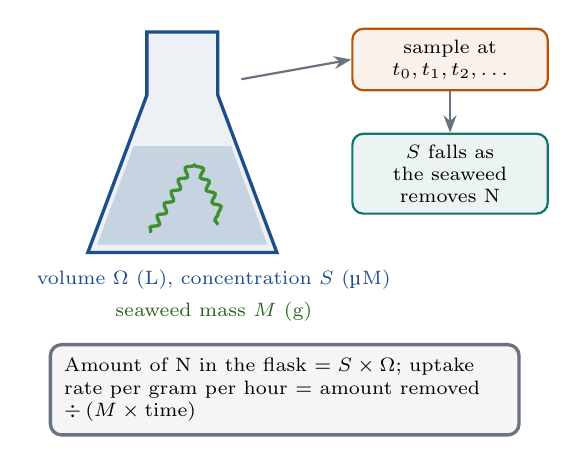
\begin{tikzpicture}[font=\scriptsize]
  \draw[very thick, sea, fill=sea!8] (-1.2,0) -- (1.2,0) -- (0.45,2.0) -- (0.45,2.8) -- (-0.45,2.8) -- (-0.45,2.0) -- cycle;
  \fill[sea!25] (-1.08,0.1) -- (1.08,0.1) -- (0.62,1.35) -- (-0.62,1.35) -- cycle;
  \draw[leaf, very thick, decorate, decoration={snake, amplitude=1.2pt, segment length=5pt}] (-0.4,0.25) -- (0.1,1.1) -- (0.45,0.35);
  \node[font=\scriptsize, sea] at (0.4,-0.35) {volume $\Omega$ (L), concentration $S$ (µM)};
  \node[font=\scriptsize, leaf!70!black] at (0.4,-0.75) {seaweed mass $M$ (g)};
  \node[flow=warm, text width=2.2cm, font=\scriptsize] (s) at (3.4,2.45) {sample at $t_0, t_1, t_2,\ldots$};
  \node[flow=accent, text width=2.2cm, font=\scriptsize] (c) at (3.4,1.0) {$S$ falls as the seaweed removes N};
  \draw[arr] (0.75,2.2) -- (s.west);
  \draw[arr] (s) -- (c);
  \node[card=grey, text width=5.6cm, font=\scriptsize, anchor=north] at (1.3,-1.15) {Amount of N in the flask $=S\times\Omega$; uptake rate per gram per hour $=$ amount removed $\div\,(M\times\text{time})$};
\end{tikzpicture}
\fignote{Schematic. Lecture 9b gives the full protocol.}}
\end{frame}

% pos 49
\begin{frame}{The multiple-flask (batch) experiment}
\centering
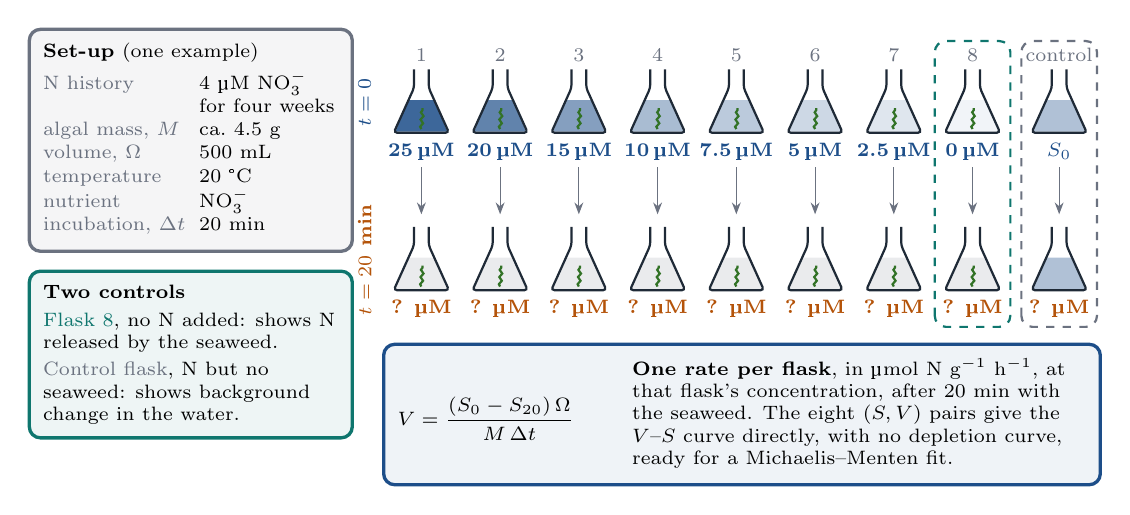
\begin{tikzpicture}[font=\scriptsize,
    flaskline/.style={ink, thick, rounded corners=1.2pt},
    weed/.style={leaf!80!black, thick, decorate, decoration={snake, amplitude=0.5pt, segment length=2.6pt}}]
  % ---- left panel: set-up and controls
  \node[card=grey, text width=3.75cm, anchor=north west, font=\scriptsize] (setup) at (-5.0,3.55) {%
    \textbf{Set-up} (one example)\\[2pt]
    \renewcommand{\arraystretch}{1.05}%
    \begin{tabular}{@{}>{\color{grey}}l@{\hspace{5pt}}l@{}}
      N history & 4 µM NO$_3^-$\\
       & for four weeks\\
      algal mass, $M$ & ca.\ 4.5 g\\
      volume, $\Omega$ & 500 mL\\
      temperature & 20 °C\\
      nutrient & NO$_3^-$\\
      incubation, $\Delta t$ & 20 min
    \end{tabular}};
  \node[card=accent, text width=3.75cm, anchor=north west, font=\scriptsize] at ([yshift=-6pt]setup.south west) {%
    \textbf{Two controls}\\[2pt]
    {\color{accent}Flask 8}, no N added: shows N released by the seaweed.\\[2pt]
    {\color{grey}Control flask}, N but no seaweed: shows background change in the water.};
  % ---- row labels
  \node[rotate=90, font=\scriptsize\bfseries, text=sea] at (-0.72,2.6) {$t = 0$};
  \node[rotate=90, font=\scriptsize\bfseries, text=warm] at (-0.72,0.6) {$t = 20$ min};
  % ---- eight treatment flasks: index / x / S0
  \foreach \i/\x/\s in {1/0/25, 2/1.0/20, 3/2.0/15, 4/3.0/10, 5/4.0/7.5, 6/5.0/5, 7/6.0/2.5, 8/7.0/0} {
    \pgfmathsetmacro{\shade}{6+3.2*\s}
    \begin{scope}[shift={(\x,2.2)}, scale=0.78]
      \fill[sea!\shade!white] (-0.42,0.04) -- (0.42,0.04) -- (0.22,0.55) -- (-0.22,0.55) -- cycle;
      \draw[weed] (0,0.08) -- (0.02,0.42);
      \draw[flaskline] (-0.12,1.05) -- (-0.12,0.75) -- (-0.45,0.02) -- (0.45,0.02) -- (0.12,0.75) -- (0.12,1.05);
    \end{scope}
    \node[font=\scriptsize, text=grey] at (\x,3.2) {\i};
    \node[font=\scriptsize\bfseries, text=sea] at (\x,1.98) {\s\,µM};
    \draw[-{Stealth[length=1.5mm]}, grey] (\x,1.78) -- (\x,1.18);
    \begin{scope}[shift={(\x,0.2)}, scale=0.78]
      \fill[grey!14] (-0.42,0.04) -- (0.42,0.04) -- (0.22,0.55) -- (-0.22,0.55) -- cycle;
      \draw[weed] (0,0.08) -- (0.02,0.42);
      \draw[flaskline] (-0.12,1.05) -- (-0.12,0.75) -- (-0.45,0.02) -- (0.45,0.02) -- (0.12,0.75) -- (0.12,1.05);
    \end{scope}
    \node[font=\scriptsize\bfseries, text=warm] at (\x,-0.02) {? µM};
  }
  \draw[accent, thick, dashed, rounded corners] (6.52,-0.25) rectangle (7.48,3.38);
  % ---- no-seaweed control
  \foreach \y/\lab/\col in {2.2/{$S_0$}/sea, 0.2/{? µM}/warm} {
    \begin{scope}[shift={(8.1,\y)}, scale=0.78]
      \fill[sea!35!white] (-0.42,0.04) -- (0.42,0.04) -- (0.22,0.55) -- (-0.22,0.55) -- cycle;
      \draw[flaskline] (-0.12,1.05) -- (-0.12,0.75) -- (-0.45,0.02) -- (0.45,0.02) -- (0.12,0.75) -- (0.12,1.05);
    \end{scope}
    \node[font=\scriptsize\bfseries, text=\col] at (8.1,\y-0.22) {\lab};
  }
  \node[font=\scriptsize, text=grey] at (8.1,3.2) {control};
  \draw[-{Stealth[length=1.5mm]}, grey] (8.1,1.78) -- (8.1,1.18);
  \draw[grey, thick, dashed, rounded corners] (7.62,-0.25) rectangle (8.58,3.38);
  % ---- rate card
  \node[card=sea, text width=8.75cm, anchor=north west, font=\scriptsize] at (-0.5,-0.45) {%
    \begin{tabular}{@{}m{2.7cm}@{\hspace{8pt}}>{\raggedright\arraybackslash}m{5.75cm}@{}}
      $V = \dfrac{(S_0 - S_{20})\,\Omega}{M\,\Delta t}$ &
      \textbf{One rate per flask}, in µmol N g$^{-1}$ h$^{-1}$, at that flask's concentration, after 20 min with the seaweed. The eight $(S, V)$ pairs give the $V$--$S$ curve directly, with no depletion curve, ready for a Michaelis--Menten fit.
    \end{tabular}};
\end{tikzpicture}
\end{frame}

% pos 50
\begin{frame}{Calculating $V$ from the multiple-flask data}
\centering
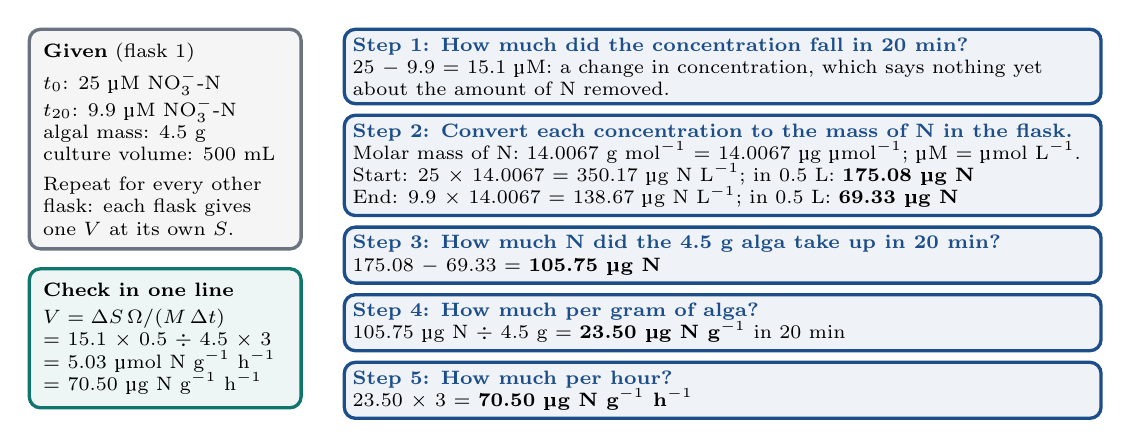
\begin{tikzpicture}[font=\scriptsize]
  \node[card=grey, text width=3.1cm, anchor=north west] (g) at (-4.0,0) {\textbf{Given} (flask 1)\\[2pt] $t_0$: 25 µM NO$_3^-$-N\\ $t_{20}$: 9.9 µM NO$_3^-$-N\\ algal mass: 4.5 g\\ culture volume: 500 mL\\[3pt] Repeat for every other flask: each flask gives one $V$ at its own $S$.};
  \node[card=accent, text width=3.1cm, anchor=north west] at ([yshift=-6pt]g.south west) {\textbf{Check in one line}\\[2pt] $V = \Delta S\,\Omega / (M\,\Delta t)$\\ = 15.1 $\times$ 0.5 $\div$ 4.5 $\times$ 3\\ = 5.03 µmol N g$^{-1}$ h$^{-1}$\\ = 70.50 µg N g$^{-1}$ h$^{-1}$};
  \node[card=sea, text width=9.4cm, anchor=north west, inner sep=3pt] (s1) at (0,0) {\textbf{\color{sea}Step 1: How much did the concentration fall in 20 min?}\\ 25 $-$ 9.9 = 15.1 µM: a change in concentration, which says nothing yet about the amount of N removed.};
  \node[card=sea, text width=9.4cm, anchor=north west, inner sep=3pt] (s2) at ([yshift=-3pt]s1.south west) {\textbf{\color{sea}Step 2: Convert each concentration to the mass of N in the flask.}\\ Molar mass of N: 14.0067 g mol$^{-1}$ = 14.0067 µg µmol$^{-1}$; µM = µmol L$^{-1}$.\\ Start: 25 $\times$ 14.0067 = 350.17 µg N L$^{-1}$; in 0.5 L: \textbf{175.08 µg N}\\ End: 9.9 $\times$ 14.0067 = 138.67 µg N L$^{-1}$; in 0.5 L: \textbf{69.33 µg N}};
  \node[card=sea, text width=9.4cm, anchor=north west, inner sep=3pt] (s3) at ([yshift=-3pt]s2.south west) {\textbf{\color{sea}Step 3: How much N did the 4.5 g alga take up in 20 min?}\\ 175.08 $-$ 69.33 = \textbf{105.75 µg N}};
  \node[card=sea, text width=9.4cm, anchor=north west, inner sep=3pt] (s4) at ([yshift=-3pt]s3.south west) {\textbf{\color{sea}Step 4: How much per gram of alga?}\\ 105.75 µg N $\div$ 4.5 g = \textbf{23.50 µg N g$^{-1}$} in 20 min};
  \node[card=sea, text width=9.4cm, anchor=north west, inner sep=3pt] (s5) at ([yshift=-3pt]s4.south west) {\textbf{\color{sea}Step 5: How much per hour?}\\ 23.50 $\times$ 3 = \textbf{70.50 µg N g$^{-1}$ h$^{-1}$}};
\end{tikzpicture}
\fignote{Rates per gram of the mass weighed into the flask; state whether it is fresh or dry mass.}
\end{frame}

% pos 51
\begin{frame}{The perturbation experiment}
\centering
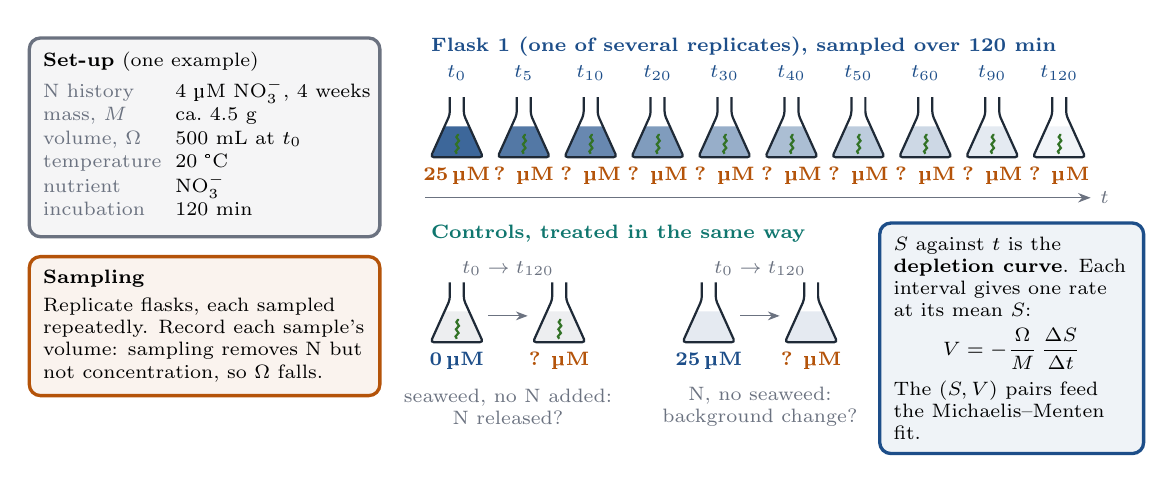
\begin{tikzpicture}[font=\scriptsize,
    flaskline/.style={ink, thick, rounded corners=1.2pt},
    weed/.style={leaf!80!black, thick, decorate, decoration={snake, amplitude=0.5pt, segment length=2.6pt}}]
  % ---- left panel: set-up and sampling
  \node[card=grey, text width=4.1cm, anchor=north west, font=\scriptsize] (setup) at (-5.45,3.55) {%
    \textbf{Set-up} (one example)\\[2pt]
    \renewcommand{\arraystretch}{1.05}%
    \begin{tabular}{@{}>{\color{grey}}l@{\hspace{5pt}}l@{}}
      N history & 4 µM NO$_3^-$, 4 weeks\\
      mass, $M$ & ca.\ 4.5 g\\
      volume, $\Omega$ & 500 mL at $t_0$\\
      temperature & 20 °C\\
      nutrient & NO$_3^-$\\
      incubation & 120 min
    \end{tabular}};
  \node[card=warm, text width=4.1cm, anchor=north west, font=\scriptsize] at ([yshift=-6pt]setup.south west) {%
    \textbf{Sampling}\\[2pt]
    Replicate flasks, each sampled repeatedly. Record each sample's volume: sampling removes N but not concentration, so $\Omega$ falls.};
  % ---- experimental flask through time: x / label / shade / S
  \node[anchor=west, font=\scriptsize\bfseries, text=sea] at (-0.45,3.42) {Flask 1 (one of several replicates), sampled over 120 min};
  \foreach \x/\t/\sh/\s in {0/0/86/{25\,µM}, 0.85/5/76/{? µM}, 1.7/10/67/{? µM}, 2.55/20/56/{? µM}, 3.4/30/46/{? µM}, 4.25/40/37/{? µM}, 5.1/50/29/{? µM}, 5.95/60/22/{? µM}, 6.8/90/12/{? µM}, 7.65/120/6/{? µM}} {
    \begin{scope}[shift={(\x,2.0)}, scale=0.74]
      \fill[sea!\sh!white] (-0.42,0.04) -- (0.42,0.04) -- (0.22,0.55) -- (-0.22,0.55) -- cycle;
      \draw[weed] (0,0.08) -- (0.02,0.42);
      \draw[flaskline] (-0.12,1.05) -- (-0.12,0.75) -- (-0.45,0.02) -- (0.45,0.02) -- (0.12,0.75) -- (0.12,1.05);
    \end{scope}
    \node[font=\scriptsize\bfseries, text=sea] at (\x,3.08) {$t_{\t}$};
    \node[font=\scriptsize\bfseries, text=warm] at (\x,1.78) {\s};
  }
  \draw[-{Stealth[length=1.6mm]}, grey] (-0.4,1.5) -- (8.05,1.5) node[right, font=\scriptsize, text=grey] {$t$};
  % ---- controls row
  \node[anchor=west, font=\scriptsize\bfseries, text=accent] at (-0.45,1.05) {Controls, treated in the same way};
  \foreach \x/\lab/\col/\sh/\w in {0/{0\,µM}/sea/0/1, 1.3/{? µM}/warm/0/1, 3.2/{25\,µM}/sea/86/0, 4.5/{? µM}/warm/86/0} {
    \begin{scope}[shift={(\x,-0.35)}, scale=0.74]
      \fill[sea!\sh!grey!12] (-0.42,0.04) -- (0.42,0.04) -- (0.22,0.55) -- (-0.22,0.55) -- cycle;
      \ifnum\w=1 \draw[weed] (0,0.08) -- (0.02,0.42); \fi
      \draw[flaskline] (-0.12,1.05) -- (-0.12,0.75) -- (-0.45,0.02) -- (0.45,0.02) -- (0.12,0.75) -- (0.12,1.05);
    \end{scope}
    \node[font=\scriptsize\bfseries, text=\col] at (\x,-0.57) {\lab};
  }
  \draw[-{Stealth[length=1.5mm]}, grey] (0.4,0.0) -- (0.9,0.0);
  \draw[-{Stealth[length=1.5mm]}, grey] (3.6,0.0) -- (4.1,0.0);
  \node[font=\scriptsize, text=grey, align=center] at (0.65,-1.15) {seaweed, no N added:\\ N released?};
  \node[font=\scriptsize, text=grey, align=center] at (3.85,-1.15) {N, no seaweed:\\ background change?};
  \node[font=\scriptsize, text=grey] at (0.65,0.6) {$t_0 \rightarrow t_{120}$};
  \node[font=\scriptsize, text=grey] at (3.85,0.6) {$t_0 \rightarrow t_{120}$};
  % ---- rate card
  \node[card=sea, text width=3.0cm, anchor=north west, font=\scriptsize] at (5.35,1.2) {%
    $S$ against $t$ is the \textbf{depletion curve}. Each interval gives one rate at its mean $S$:\\[3pt]
    \centering $V = -\dfrac{\Omega}{M}\,\dfrac{\Delta S}{\Delta t}$\\[3pt]
    \raggedright The $(S, V)$ pairs feed the Michaelis--Menten fit.};
\end{tikzpicture}
\end{frame}

% pos 52
\begin{frame}{From a depletion curve to an uptake rate}
\twocol{
\begin{itemize}
  \item During depletion the slope $\Delta S/\Delta t$ is negative
  \item Correct for water volume $\Omega$ and algal mass $M$:
  \[ V = -\frac{\Omega}{M}\,\frac{\Delta S}{\Delta t} \]
  \item Use hours for $\Delta t$ to report µmol N g$^{-1}$ h$^{-1}$
  \item The slope is steepest at the start, when $S$ is highest
  \item Different uptake properties give differently shaped curves
\end{itemize}}{
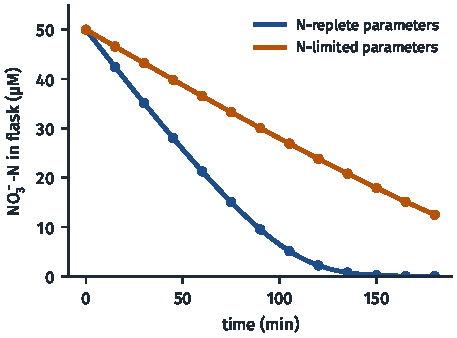
\includegraphics[width=0.95\linewidth]{fig_depletion}
\fignote{Modelled depletion for 0.5 g dry mass in 0.5 L, using the Michaelis–Menten parameters for N-replete and N-limited \textit{Gracilaria gracilis} at 15\,°C (Smit 2002, Table II).}}
\end{frame}

% pos 53
\begin{frame}{From samples to a depletion curve}
\centering
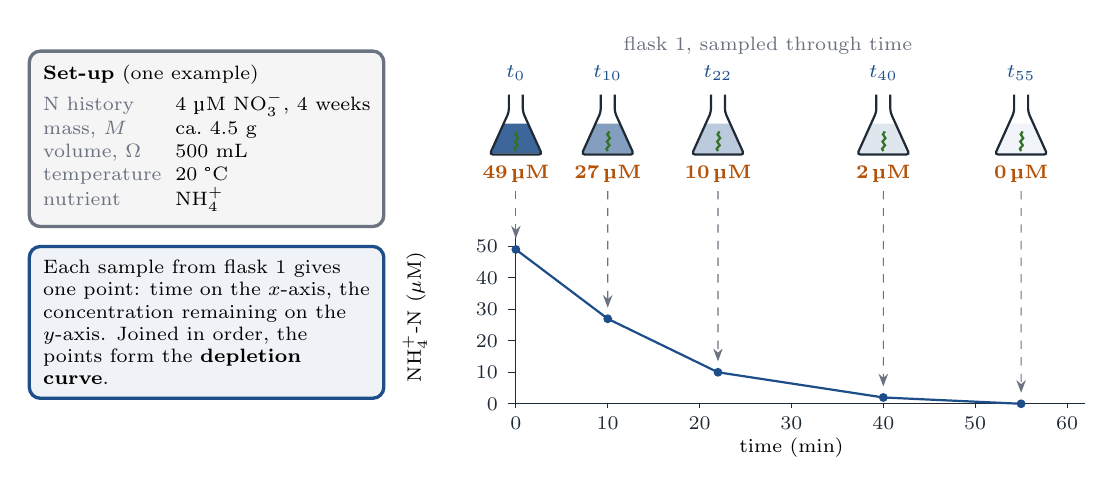
\begin{tikzpicture}[font=\scriptsize,
    flaskline/.style={ink, thick, rounded corners=1.2pt},
    weed/.style={leaf!80!black, thick, decorate, decoration={snake, amplitude=0.5pt, segment length=2.6pt}}]
  % ---- set-up
  \node[card=grey, text width=4.15cm, anchor=north west] (setup) at (-6.2,2.6) {%
    \textbf{Set-up} (one example)\\[2pt]
    \renewcommand{\arraystretch}{1.05}%
    \begin{tabular}{@{}>{\color{grey}}l@{\hspace{5pt}}l@{}}
      N history & 4 µM NO$_3^-$, 4 weeks\\
      mass, $M$ & ca.\ 4.5 g\\
      volume, $\Omega$ & 500 mL\\
      temperature & 20 °C\\
      nutrient & NH$_4^+$
    \end{tabular}};
  \node[card=sea, text width=4.15cm, anchor=north west] at ([yshift=-6pt]setup.south west) {%
    Each sample from flask 1 gives one point: time on the $x$-axis, the concentration remaining on the $y$-axis. Joined in order, the points form the \textbf{depletion curve}.};
  % ---- axes: origin (0,-1.9); 1 min = 7/60 cm
  \begin{scope}[shift={(0,-1.9)}, x=0.11667cm, y=0.04cm]
    \draw[ink] (0,57) -- (0,0) -- (62,0);
    \foreach \v in {0,10,...,60} {\draw[ink] (\v,0) -- (\v,-1.2) node[below, font=\scriptsize] {\v};}
    \foreach \v in {0,10,20,30,40,50} {\draw[ink] (0,\v) -- (-0.9,\v) node[left, font=\scriptsize] {\v};}
    \node[font=\scriptsize] at (30,-14) {time (min)};
    \node[font=\scriptsize, rotate=90] at (-11,27.5) {NH$_4^+$-N ($\mu$M)};
    \draw[thick, sea] (0,49) -- (10,27) -- (22,10) -- (40,2) -- (55,0);
    \foreach \tt/\ss [count=\k] in {0/49, 10/27, 22/10, 40/2, 55/0} {\fill[sea] (\tt,\ss) circle (1.6pt); \coordinate (p\k) at (\tt,\ss);}
  \end{scope}
  % ---- flask 1 at each sampling time, above its own time
  \foreach \x/\t/\s/\sh [count=\k] in {0/0/49/86, 1.1667/10/27/55, 2.5667/22/10/30, 4.6667/40/2/14, 6.4167/55/0/6} {
    \begin{scope}[shift={(\x,1.25)}, scale=0.74]
      \fill[sea!\sh!white] (-0.42,0.04) -- (0.42,0.04) -- (0.22,0.55) -- (-0.22,0.55) -- cycle;
      \draw[weed] (0,0.08) -- (0.02,0.42);
      \draw[flaskline] (-0.12,1.05) -- (-0.12,0.75) -- (-0.45,0.02) -- (0.45,0.02) -- (0.12,0.75) -- (0.12,1.05);
    \end{scope}
    \node[font=\scriptsize\bfseries, text=sea] at (\x,2.3) {$t_{\t}$};
    \node[font=\scriptsize\bfseries, text=warm] at (\x,1.02) {\s\,µM};
    \draw[-{Stealth[length=1.6mm]}, grey, dashed] (\x,0.8) -- ([yshift=4pt]p\k);
  }
  \node[font=\scriptsize, text=grey] at (3.2,2.65) {flask 1, sampled through time};
\end{tikzpicture}
\fignote{Example values for one flask of N-replete \textit{Gracilaria gracilis} (after Smit 2002).}
\end{frame}

% pos 54
\begin{frame}{From a depletion curve to uptake rates}
\centering
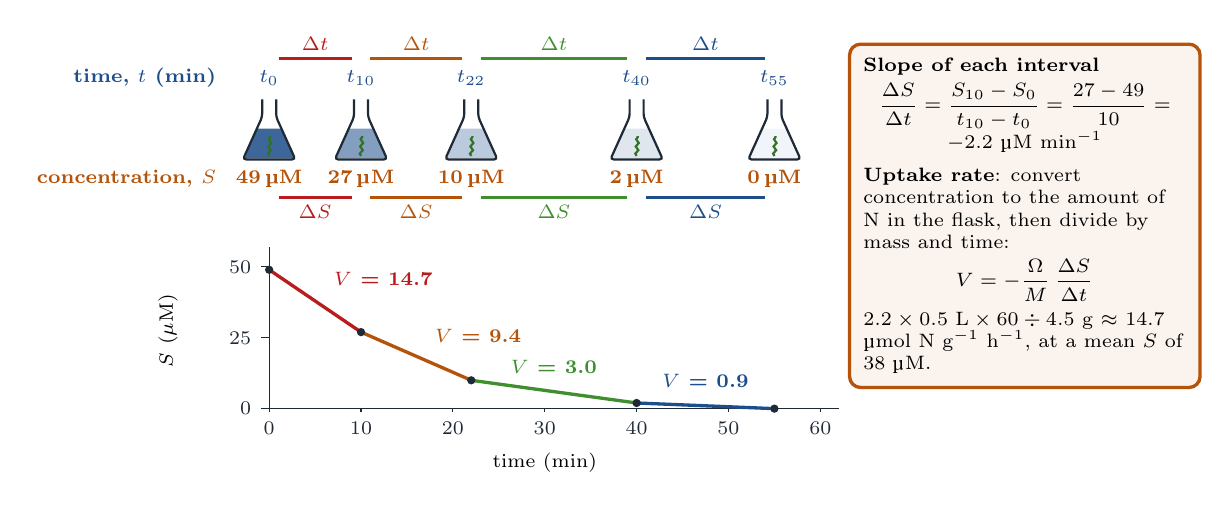
\begin{tikzpicture}[font=\scriptsize,
    flaskline/.style={ink, thick, rounded corners=1.2pt},
    weed/.style={leaf!80!black, thick, decorate, decoration={snake, amplitude=0.5pt, segment length=2.6pt}}]
  % ---- axes: origin (0,-1.9); 1 min = 7/60 cm
  \begin{scope}[shift={(0,-1.9)}, x=0.11667cm, y=0.036cm]
    \draw[ink] (0,57) -- (0,0) -- (62,0);
    \foreach \v in {0,10,...,60} {\draw[ink] (\v,0) -- (\v,-1.2) node[below, font=\scriptsize] {\v};}
    \foreach \v in {0,25,50} {\draw[ink] (0,\v) -- (-0.9,\v) node[left, font=\scriptsize] {\v};}
    \node[font=\scriptsize] at (30,-19) {time (min)};
    \node[font=\scriptsize, rotate=90] at (-11,27.5) {$S$ ($\mu$M)};
    \draw[very thick, hot] (0,49) -- (10,27); \draw[very thick, warm] (10,27) -- (22,10);
    \draw[very thick, leaf] (22,10) -- (40,2); \draw[very thick, sea] (40,2) -- (55,0);
    \foreach \tt/\ss in {0/49, 10/27, 22/10, 40/2, 55/0} {\fill[ink] (\tt,\ss) circle (1.5pt);}
    % V per interval = -(dS/dt) x 60 x 0.5 L / 4.5 g
    \node[hot, anchor=south west, font=\scriptsize\bfseries] at (6,40) {$V$ = 14.7};
    \node[warm, anchor=south west, font=\scriptsize\bfseries] at (17,20) {$V$ = 9.4};
    \node[leaf, anchor=south, font=\scriptsize\bfseries] at (31,9) {$V$ = 3.0};
    \node[sea, anchor=south, font=\scriptsize\bfseries] at (47.5,4) {$V$ = 0.9};
  \end{scope}
  % ---- row labels
  \node[font=\scriptsize\bfseries, text=sea, anchor=east] at (-0.55,2.3) {time, $t$ (min)};
  \node[font=\scriptsize\bfseries, text=warm, anchor=east] at (-0.55,1.02) {concentration, $S$};
  % ---- flasks
  \foreach \x/\t/\s/\sh in {0/0/49/86, 1.1667/10/27/55, 2.5667/22/10/30, 4.6667/40/2/14, 6.4167/55/0/6} {
    \begin{scope}[shift={(\x,1.25)}, scale=0.74]
      \fill[sea!\sh!white] (-0.42,0.04) -- (0.42,0.04) -- (0.22,0.55) -- (-0.22,0.55) -- cycle;
      \draw[weed] (0,0.08) -- (0.02,0.42);
      \draw[flaskline] (-0.12,1.05) -- (-0.12,0.75) -- (-0.45,0.02) -- (0.45,0.02) -- (0.12,0.75) -- (0.12,1.05);
    \end{scope}
    \node[font=\scriptsize\bfseries, text=sea] at (\x,2.3) {$t_{\t}$};
    \node[font=\scriptsize\bfseries, text=warm] at (\x,1.02) {\s\,µM};
  }
  % ---- interval brackets: Delta t above, Delta S below, coloured as the secants
  \foreach \a/\b/\c in {0/1.1667/hot, 1.1667/2.5667/warm, 2.5667/4.6667/leaf, 4.6667/6.4167/sea} {
    \draw[\c, very thick] (\a+0.12,2.55) -- (\b-0.12,2.55) node[midway, above=-1pt, font=\scriptsize] {$\Delta t$};
    \draw[\c, very thick] (\a+0.12,0.78) -- (\b-0.12,0.78) node[midway, below=-1pt, font=\scriptsize] {$\Delta S$};
  }
  % ---- calculation card
  \node[card=warm, text width=4.1cm, anchor=north west] at (7.35,2.75) {%
    \textbf{Slope of each interval}\\[2pt]
    \centering $\dfrac{\Delta S}{\Delta t} = \dfrac{S_{10} - S_0}{t_{10} - t_0} = \dfrac{27 - 49}{10} = -2.2$ µM min$^{-1}$\\[4pt]
    \raggedright\textbf{Uptake rate}: convert concentration to the amount of N in the flask, then divide by mass and time:\\[3pt]
    \centering $V = -\dfrac{\Omega}{M}\,\dfrac{\Delta S}{\Delta t}$\\[3pt]
    \raggedright $2.2 \times 0.5\ \text{L} \times 60 \div 4.5$ g $\approx$ 14.7 µmol N g$^{-1}$ h$^{-1}$, at a mean $S$ of 38 µM.};
\end{tikzpicture}
\fignote{$V$ in µmol N g$^{-1}$ h$^{-1}$. The worked rates ignore sample removal (Lab 4 corrects for it).}
\end{frame}

% pos 55
\begin{frame}{Calculating $V$ from a depletion curve}
\centering
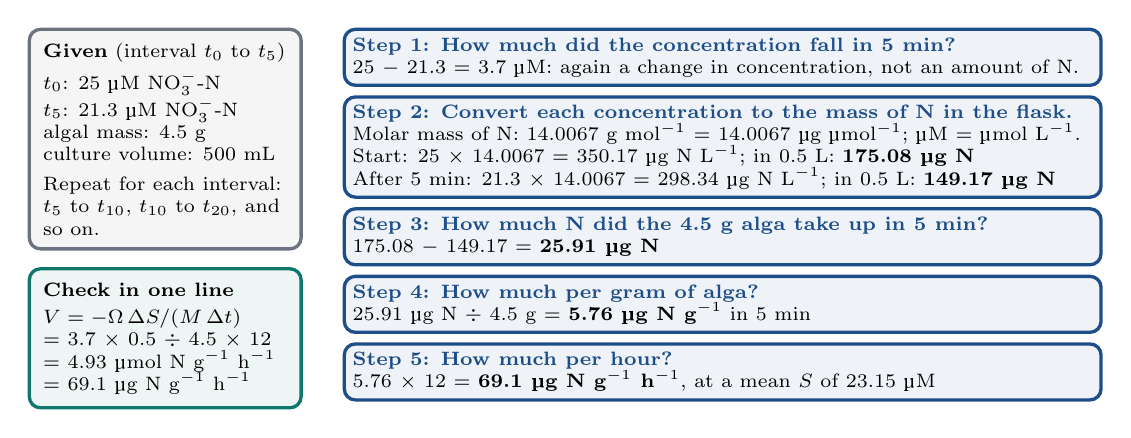
\begin{tikzpicture}[font=\scriptsize]
  \node[card=grey, text width=3.1cm, anchor=north west] (g) at (-4.0,0) {\textbf{Given} (interval $t_0$ to $t_5$)\\[2pt] $t_0$: 25 µM NO$_3^-$-N\\ $t_5$: 21.3 µM NO$_3^-$-N\\ algal mass: 4.5 g\\ culture volume: 500 mL\\[3pt] Repeat for each interval: $t_5$ to $t_{10}$, $t_{10}$ to $t_{20}$, and so on.};
  \node[card=accent, text width=3.1cm, anchor=north west] at ([yshift=-6pt]g.south west) {\textbf{Check in one line}\\[2pt] $V = -\Omega\,\Delta S / (M\,\Delta t)$\\ = 3.7 $\times$ 0.5 $\div$ 4.5 $\times$ 12\\ = 4.93 µmol N g$^{-1}$ h$^{-1}$\\ = 69.1 µg N g$^{-1}$ h$^{-1}$};
  \node[card=sea, text width=9.4cm, anchor=north west, inner sep=3pt] (s1) at (0,0) {\textbf{\color{sea}Step 1: How much did the concentration fall in 5 min?}\\ 25 $-$ 21.3 = 3.7 µM: again a change in concentration, not an amount of N.};
  \node[card=sea, text width=9.4cm, anchor=north west, inner sep=3pt] (s2) at ([yshift=-3pt]s1.south west) {\textbf{\color{sea}Step 2: Convert each concentration to the mass of N in the flask.}\\ Molar mass of N: 14.0067 g mol$^{-1}$ = 14.0067 µg µmol$^{-1}$; µM = µmol L$^{-1}$.\\ Start: 25 $\times$ 14.0067 = 350.17 µg N L$^{-1}$; in 0.5 L: \textbf{175.08 µg N}\\ After 5 min: 21.3 $\times$ 14.0067 = 298.34 µg N L$^{-1}$; in 0.5 L: \textbf{149.17 µg N}};
  \node[card=sea, text width=9.4cm, anchor=north west, inner sep=3pt] (s3) at ([yshift=-3pt]s2.south west) {\textbf{\color{sea}Step 3: How much N did the 4.5 g alga take up in 5 min?}\\ 175.08 $-$ 149.17 = \textbf{25.91 µg N}};
  \node[card=sea, text width=9.4cm, anchor=north west, inner sep=3pt] (s4) at ([yshift=-3pt]s3.south west) {\textbf{\color{sea}Step 4: How much per gram of alga?}\\ 25.91 µg N $\div$ 4.5 g = \textbf{5.76 µg N g$^{-1}$} in 5 min};
  \node[card=sea, text width=9.4cm, anchor=north west, inner sep=3pt] (s5) at ([yshift=-3pt]s4.south west) {\textbf{\color{sea}Step 5: How much per hour?}\\ 5.76 $\times$ 12 = \textbf{69.1 µg N g$^{-1}$ h$^{-1}$}, at a mean $S$ of 23.15 µM};
\end{tikzpicture}
\fignote{Each interval gives one $(S, V)$ pair. Sampling removes water, so later intervals use the volume remaining (Lab 4).}
\end{frame}

% pos 56
\begin{frame}{Uptake mechanisms}
\begin{center}
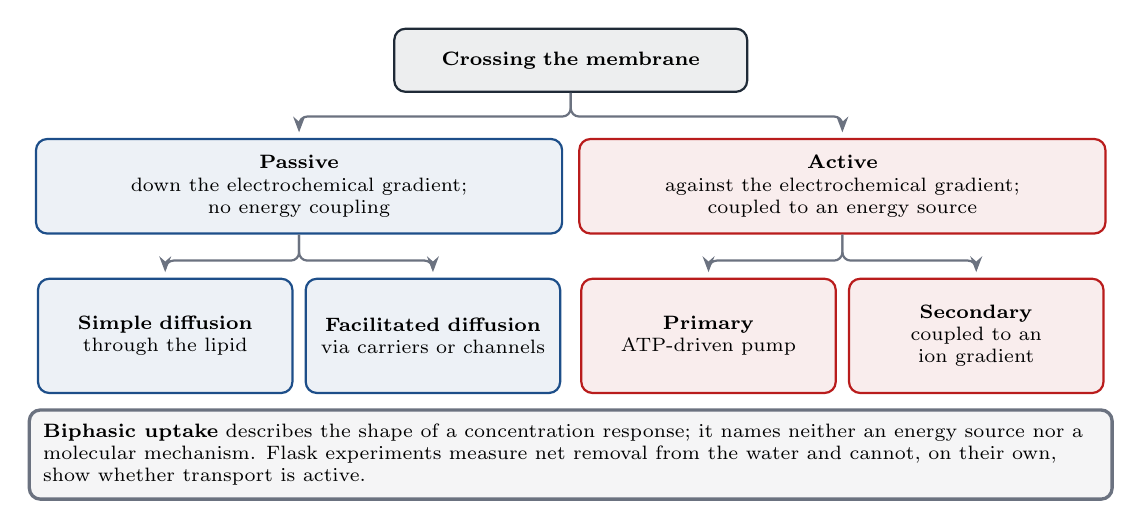
\begin{tikzpicture}[font=\scriptsize,
    lvl/.style={text width=6.4cm, minimum height=1.2cm},
    leaf/.style={text width=2.95cm, minimum height=1.45cm, font=\scriptsize},
    elbow/.style={-{Stealth[length=2mm]}, thick, grey, rounded corners=3pt, shorten >=2pt}]
  \node[flow=ink, text width=4.2cm, minimum height=0.8cm] (m) at (0,0) {\textbf{Crossing the membrane}};
  \node[flow=sea, lvl] (p) at (-3.45,-1.6) {\textbf{Passive}\\ down the electrochemical gradient;\\ no energy coupling};
  \node[flow=hot, lvl] (a) at (3.45,-1.6) {\textbf{Active}\\ against the electrochemical gradient;\\ coupled to an energy source};
  \node[flow=sea, leaf] (sd) at (-5.15,-3.5) {\textbf{Simple diffusion}\\ through the lipid};
  \node[flow=sea, leaf] (fd) at (-1.75,-3.5) {\textbf{Facilitated diffusion}\\ via carriers or channels};
  \node[flow=hot, leaf] (pr) at (1.75,-3.5) {\textbf{Primary}\\ ATP-driven pump};
  \node[flow=hot, leaf] (se) at (5.15,-3.5) {\textbf{Secondary}\\ coupled to an ion gradient};
  \foreach \c in {p,a} \draw[elbow] (m.south) -- ++(0,-0.3) -| (\c.north);
  \foreach \c in {sd,fd} \draw[elbow] (p.south) -- ++(0,-0.33) -| (\c.north);
  \foreach \c in {pr,se} \draw[elbow] (a.south) -- ++(0,-0.33) -| (\c.north);
  \node[card=grey, text width=13.4cm, font=\scriptsize, anchor=north] at (0,-4.42) {\textbf{Biphasic uptake} describes the shape of a concentration response; it names neither an energy source nor a molecular mechanism. Flask experiments measure net removal from the water and cannot, on their own, show whether transport is active.};
\end{tikzpicture}
\end{center}
\end{frame}

% pos 57
\begin{frame}{Uptake kinetics: $V$ against $S$}
\twocol{
\begin{itemize}
  \item Plot uptake rate ($V$) against substrate concentration ($S$)
  \item A saturable system can follow the Michaelis–Menten equation, borrowed from enzyme kinetics
  \item High $S$: $V$ approaches a limiting capacity
  \item Low $S$: uptake sites are unoccupied more of the time, so $V$ falls
  \item A falling rate alone does not demonstrate diffusion limitation
  \item The model assumes one-way uptake, with no losses after uptake
\end{itemize}}{
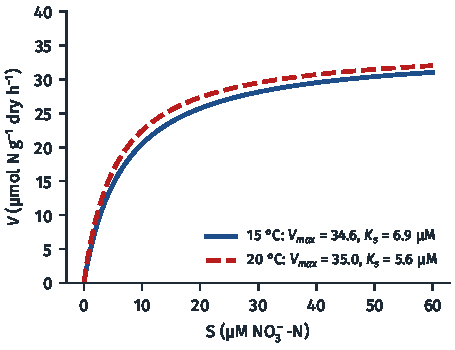
\includegraphics[width=0.95\linewidth]{fig_mm_nitrate}
\fignote{Model curves for nitrate uptake by N-replete \textit{Gracilaria gracilis} at 15 and 20\,°C (Smit 2002, Table II).}}
\end{frame}

% pos 58
\begin{frame}{The Michaelis–Menten model}
\twocol{
\begin{itemize}
  \item $V_\text{max}$: the limiting uptake capacity under the stated conditions
  \item $K_s$: the half-saturation concentration; at $S=K_s$, $V=V_\text{max}/2$
  \item $V$ approaches $V_\text{max}$ asymptotically and never reaches it at a finite $S$
  \item Perturbation experiment: closest to $V_\text{max}$ at the start; multiple flasks: in the highest-concentration flasks
\end{itemize}}{
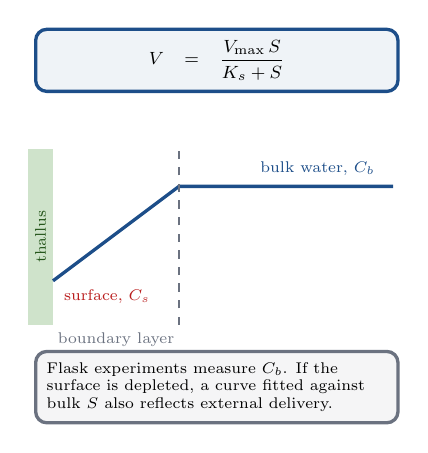
\begin{tikzpicture}[font=\scriptsize, scale=0.8, transform shape]
  \node[card=sea, text width=5.4cm, align=center] (eq) at (0,1.6) {\footnotesize $V = \dfrac{V_\text{max}\, S}{K_s + S}$};
  \fill[leaf!25] (-3.0,-2.6) rectangle (-2.6,0.2);
  \node[rotate=90, font=\scriptsize, leaf!60!black] at (-2.8,-1.2) {thallus};
  \draw[very thick, sea] (-2.6,-1.9) -- (-0.6,-0.4) -- (2.8,-0.4);
  \draw[grey, dashed] (-0.6,-2.6) -- (-0.6,0.2);
  \node[font=\scriptsize, sea, anchor=south] at (1.6,-0.35) {bulk water, $C_b$};
  \node[font=\scriptsize, hot, anchor=west] at (-2.55,-2.15) {surface, $C_s$};
  \node[font=\scriptsize, grey, anchor=north] at (-1.6,-2.6) {boundary layer};
  \node[card=grey, text width=5.4cm, font=\scriptsize, anchor=north] at (0,-3.0) {Flask experiments measure $C_b$. If the surface is depleted, a curve fitted against bulk $S$ also reflects external delivery.};
\end{tikzpicture}
\fignote{Schematic concentration profile.}}
\end{frame}

% pos 59
\begin{frame}{From the depletion curve to the $V$--$S$ curve}
\centering
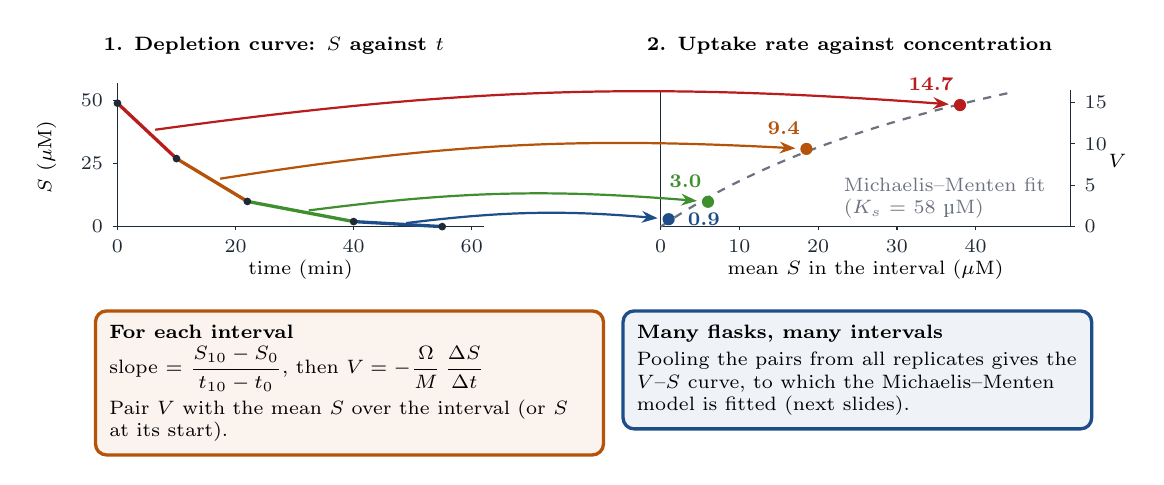
\begin{tikzpicture}[font=\scriptsize]
  % ---- panel 1: depletion curve (S against t)
  \node[font=\scriptsize\bfseries, anchor=west] at (-0.3,2.3) {1. Depletion curve: $S$ against $t$};
  \begin{scope}[x=0.075cm, y=0.032cm]
    \draw[ink] (0,57) -- (0,0) -- (62,0);
    \foreach \v in {0,20,40,60} {\draw[ink] (\v,0) -- (\v,-1.5) node[below] {\v};}
    \foreach \v in {0,25,50} {\draw[ink] (0,\v) -- (-0.8,\v) node[left] {\v};}
    \node at (31,-17) {time (min)};
    \node[rotate=90] at (-12,27.5) {$S$ ($\mu$M)};
    \draw[very thick, hot] (0,49) -- (10,27);
    \draw[very thick, warm] (10,27) -- (22,10);
    \draw[very thick, leaf] (22,10) -- (40,2);
    \draw[very thick, sea] (40,2) -- (55,0);
    \fill[ink] (0,49) circle (1.4pt);
    \fill[ink] (10,27) circle (1.4pt);
    \fill[ink] (22,10) circle (1.4pt);
    \fill[ink] (40,2) circle (1.4pt);
    \fill[ink] (55,0) circle (1.4pt);
    \coordinate (m0) at (5.0,38.0);
    \coordinate (m1) at (16.0,18.5);
    \coordinate (m2) at (31.0,6.0);
    \coordinate (m3) at (47.5,1.0);
  \end{scope}
  % ---- panel 2: V against S
  \node[font=\scriptsize\bfseries, anchor=west] at (6.6,2.3) {2. Uptake rate against concentration};
  \begin{scope}[shift={(6.9,0)}, x=0.1cm, y=0.105cm]
    \draw[ink] (0,16.5) -- (0,0) -- (52,0) -- (52,16.5);
    \foreach \v in {0,10,...,40} {\draw[ink] (\v,0) -- (\v,-0.4) node[below] {\v};}
    \foreach \v in {0,5,10,15} {\draw[ink] (52,\v) -- (52.6,\v) node[right] {\v};}
    \node at (26,-5.2) {mean $S$ in the interval ($\mu$M)};
    \node at (58,8) {$V$};
        % least-squares Michaelis-Menten fit to the four points: Vmax 37.2, Ks 57.5 uM
    \draw[grey, thick, dashed, domain=0:45, samples=60] plot (\x,{37.21*\x/(57.53+\x)});
    \node[grey, anchor=west, align=left, font=\scriptsize] at (22,3.4) {Michaelis--Menten fit\\ ($K_s$ = 58 µM)};
    \fill[hot] (38.0,14.7) circle (2.2pt); \coordinate (v0) at (38.0,14.7);
    \node[hot, anchor=south east, font=\scriptsize\bfseries] at (38.400000000000006,15.299999999999999) {14.7};
    \fill[warm] (18.5,9.4) circle (2.2pt); \coordinate (v1) at (18.5,9.4);
    \node[warm, anchor=south east, font=\scriptsize\bfseries] at (18.9,10.0) {9.4};
    \fill[leaf] (6.0,3.0) circle (2.2pt); \coordinate (v2) at (6.0,3.0);
    \node[leaf, anchor=south east, font=\scriptsize\bfseries] at (6.4,3.6) {3.0};
    \fill[sea] (1.0,0.9) circle (2.2pt); \coordinate (v3) at (1.0,0.9);
    \node[sea, anchor=west, font=\scriptsize\bfseries] at (2.2,0.9) {0.9};
  \end{scope}
  \draw[-{Stealth[length=2mm]}, hot, thick, shorten <=3pt, shorten >=4pt] (m0) to[bend left=6] (v0);
  \draw[-{Stealth[length=2mm]}, warm, thick, shorten <=3pt, shorten >=4pt] (m1) to[bend left=6] (v1);
  \draw[-{Stealth[length=2mm]}, leaf, thick, shorten <=3pt, shorten >=4pt] (m2) to[bend left=6] (v2);
  \draw[-{Stealth[length=2mm]}, sea, thick, shorten <=3pt, shorten >=4pt] (m3) to[bend left=6] (v3);
  % ---- explanation
  \node[card=warm, text width=6.1cm, anchor=north west] at (-0.3,-1.05) {\textbf{For each interval}\\[2pt]
    slope = $\dfrac{S_{10} - S_0}{t_{10} - t_0}$, then $V = -\dfrac{\Omega}{M}\,\dfrac{\Delta S}{\Delta t}$\\[2pt]
    Pair $V$ with the mean $S$ over the interval (or $S$ at its start).};
  \node[card=sea, text width=5.6cm, anchor=north west] at (6.4,-1.05) {\textbf{Many flasks, many intervals}\\[2pt]
    Pooling the pairs from all replicates gives the $V$--$S$ curve, to which the Michaelis--Menten model is fitted (next slides).};
\end{tikzpicture}
\fignote{Example values as on the previous slides (0.5 L, 4.5 g); $V$ in µmol N g$^{-1}$ h$^{-1}$.}
\end{frame}

% pos 60
\begin{frame}{Reading the Michaelis–Menten graph}
\twocol{
\begin{itemize}
  \item $V_\text{max}$: limiting rate, on a stated biomass or area basis
  \item $K_s$: concentration at half the limiting rate; generally not an equilibrium binding constant
  \item $\alpha$: the initial slope, $\alpha = V_\text{max}/K_s$
  \item At high $S$, doubling $S$ adds little uptake
  \item At low $S$, a change in $S$ has a large proportional effect
\end{itemize}}{
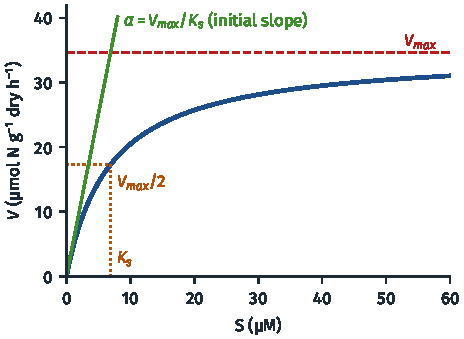
\includegraphics[width=0.95\linewidth]{fig_mm_params}
\fignote{Parameters for nitrate uptake by N-replete \textit{Gracilaria gracilis} at 15\,°C: $V_\text{max}$ = 34.6 µmol N g$^{-1}$ dry h$^{-1}$, $K_s$ = 6.9 µM (Smit 2002, Table II).}}
\end{frame}

% pos 61
\begin{frame}{Comparing uptake at low concentration}
\twocol{
\begin{itemize}
  \item $V_\text{max}$, $K_s$ and $\alpha$ allow comparisons among species and conditions measured the same way
  \item At equal $V_\text{max}$, a lower $K_s$ gives a steeper initial slope
  \item When capacities differ, compare $\alpha$, not $K_s$ alone
  \item Example: A ($V_\text{max}$ 4, $K_s$ 1) and B ($V_\text{max}$ 12, $K_s$ 2); at $S$ = 0.5, A takes up 1.33 and B 2.40
  \item Parameters depend on physiology, SA:V, light, temperature and history
\end{itemize}}{
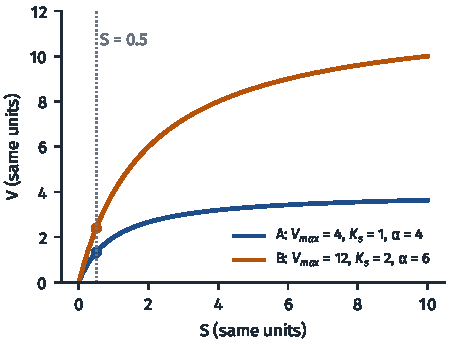
\includegraphics[width=0.95\linewidth]{fig_alpha_ab}
\fignote{Worked example from the notes; same units and biomass basis for both populations.}}
\end{frame}

% pos 62
\begin{frame}{From depletion slopes to the $V$–$S$ hyperbola}
\begin{center}
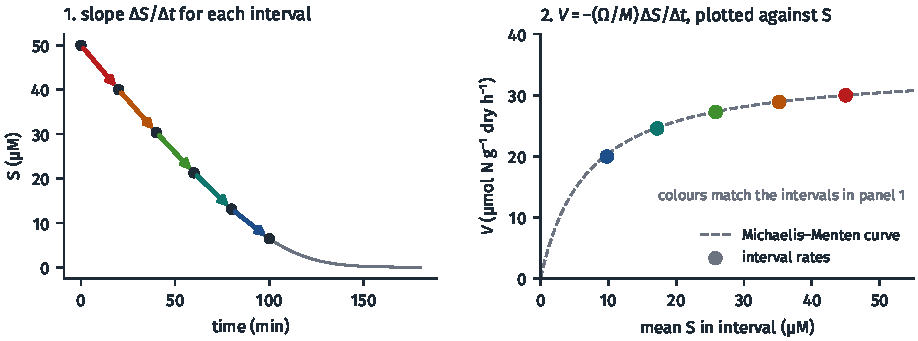
\includegraphics[width=0.86\textwidth]{fig_slope_to_v}
\end{center}
\vspace{-4pt}
{\footnotesize Each interval gives one rate at its mean concentration. A rectangular hyperbola is consistent with a saturable system: active transport or passive facilitated transport. The curve describes the concentration response; the mechanism needs other evidence.}
\fignote{Modelled flask: 0.5 g dry mass in 0.5 L, N-replete parameters at 15\,°C (Smit 2002, Table II); 20-min sampling.}
\end{frame}

% pos 63
\begin{frame}{Active uptake}
\twocol{
\begin{itemize}
  \item Moves a nutrient \textbf{against its electrochemical gradient}
  \item Requires coupling to an energy source, directly (ATP) or through another ion's gradient
  \item For an ion, both concentration and membrane voltage set the gradient
  \item A concentration difference alone does not identify uphill transport
\end{itemize}}{
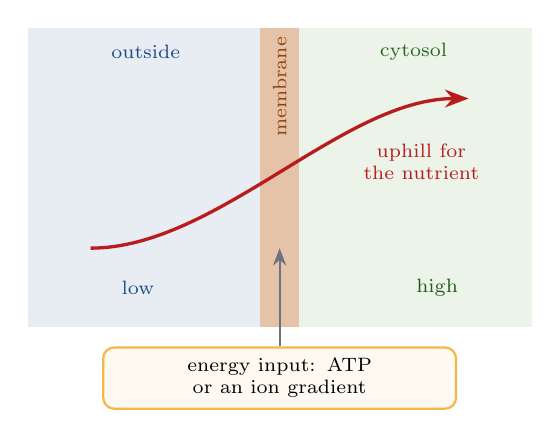
\begin{tikzpicture}[font=\scriptsize]
  \fill[sea!10] (-3.2,-1.9) rectangle (-0.25,1.9);
  \fill[leaf!10] (0.25,-1.9) rectangle (3.2,1.9);
  \fill[warm!35] (-0.25,-1.9) rectangle (0.25,1.9);
  \node[font=\scriptsize, sea] at (-1.7,1.6) {outside};
  \node[font=\scriptsize, leaf!70!black] at (1.7,1.6) {cytosol};
  \node[font=\scriptsize, warm!80!black, rotate=90] at (0,1.15) {membrane};
  \draw[very thick, hot, -{Stealth[length=3mm]}] (-2.4,-0.9) .. controls (-0.8,-0.9) and (0.8,1.0) .. (2.4,1.0);
  \node[font=\scriptsize, hot, align=center] at (1.8,0.2) {uphill for\\ the nutrient};
  \node[flow=sand, font=\scriptsize, text width=4.2cm] (e) at (0,-2.55) {energy input: ATP or an ion gradient};
  \draw[arr] (e.north) -- (0,-0.9);
  \node[font=\scriptsize, sea, align=center] at (-1.8,-1.4) {low};
  \node[font=\scriptsize, leaf!60!black, align=center] at (2.0,-1.4) {high};
\end{tikzpicture}
\fignote{Schematic.}}
\end{frame}

% pos 64
\begin{frame}{Concentrations on either side of the membrane}
\twocol{
\begin{itemize}
  \item External dissolved N: often in the \textbf{micromolar} range
  \item Some internal pools: up to the \textbf{millimolar} range
  \item Compare the same free dissolved species on both sides
  \item Total tissue N includes organic compounds and several compartments; it is not free cytosolic nitrate
  \item Moving uphill requires active transport; passive routes work where the gradient is favourable
\end{itemize}}{
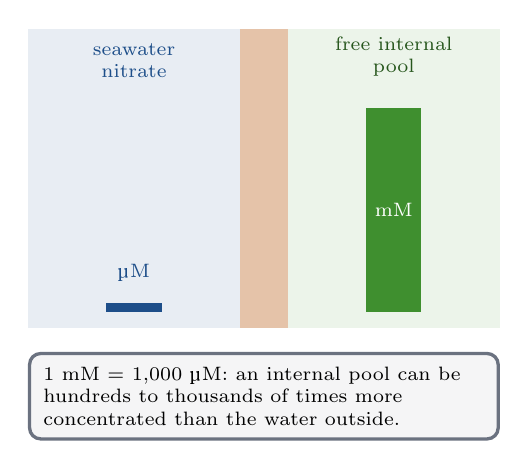
\begin{tikzpicture}[font=\scriptsize]
  \fill[sea!10] (-3.0,-0.2) rectangle (-0.3,3.6);
  \fill[leaf!10] (0.3,-0.2) rectangle (3.0,3.6);
  \fill[warm!35] (-0.3,-0.2) rectangle (0.3,3.6);
  \fill[sea] (-2.0,0) rectangle (-1.3,0.12);
  \fill[leaf] (1.3,0) rectangle (2.0,2.6);
  \node[font=\scriptsize, sea] at (-1.65,0.5) {µM};
  \node[font=\scriptsize, white] at (1.65,1.3) {mM};
  \node[font=\scriptsize, sea, align=center] at (-1.65,3.2) {seawater\\ nitrate};
  \node[font=\scriptsize, leaf!60!black, align=center] at (1.65,3.25) {free internal\\ pool};
  \node[card=grey, text width=5.6cm, font=\scriptsize, anchor=north] at (0,-0.5) {1 mM = 1,000 µM: an internal pool can be hundreds to thousands of times more concentrated than the water outside.};
\end{tikzpicture}
\fignote{Schematic; bar heights not to scale.}}
\end{frame}

% pos 63_
\begin{frame}{Primary and secondary active transport}
\twocol{
\begin{itemize}
  \item \textbf{Primary}: an H$^+$-ATPase uses ATP to export H$^+$, building a voltage and a pH difference
  \item \textbf{Secondary}: H$^+$ flowing back in through a carrier drives nitrate in with it; the carrier does not hydrolyse ATP
  \item \textbf{Symport}: coupled substances cross the same protein in the same direction
  \item \textbf{Antiport}: they cross the same protein in opposite directions
  \item ATP comes from metabolism; uptake need not stop the moment light does
\end{itemize}}{
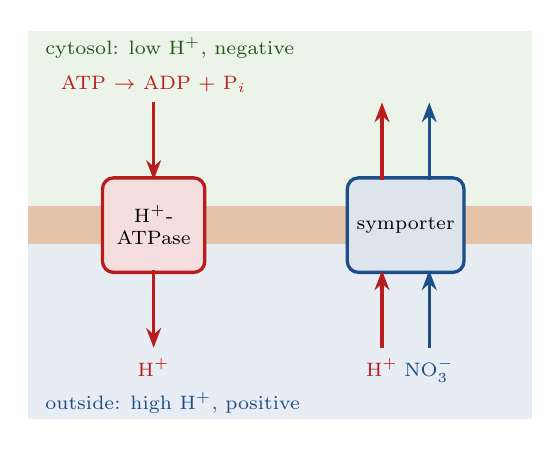
\begin{tikzpicture}[font=\scriptsize, yscale=0.82]
  \fill[sea!10] (-3.2,-3.0) rectangle (3.2,-0.3);
  \fill[leaf!10] (-3.2,0.3) rectangle (3.2,3.0);
  \fill[warm!35] (-3.2,-0.3) rectangle (3.2,0.3);
  \node[font=\scriptsize, sea, anchor=west] at (-3.1,-2.75) {outside: high H$^+$, positive};
  \node[font=\scriptsize, leaf!60!black, anchor=west] at (-3.1,2.75) {cytosol: low H$^+$, negative};
  \node[draw=hot, very thick, fill=hot!15, rounded corners, minimum width=1.3cm, minimum height=1.2cm, font=\scriptsize, align=center] (pump) at (-1.6,0) {H$^+$-\\ATPase};
  \node[draw=sea, very thick, fill=sea!15, rounded corners, minimum width=1.3cm, minimum height=1.2cm, font=\scriptsize, align=center] (sym) at (1.6,0) {symporter};
  \draw[very thick, hot, -{Stealth[length=2.5mm]}] (-1.6,1.9) -- (-1.6,0.7);
  \draw[very thick, hot, -{Stealth[length=2.5mm]}] (-1.6,-0.7) -- (-1.6,-1.9) node[below, font=\scriptsize] {H$^+$};
  \node[font=\scriptsize, hot, anchor=south] at (-1.6,1.9) {ATP $\rightarrow$ ADP + P$_i$};
  \draw[very thick, hot, -{Stealth[length=2.5mm]}] (1.3,-1.9) node[below, font=\scriptsize] {H$^+$} -- (1.3,-0.7);
  \draw[very thick, hot, -{Stealth[length=2.5mm]}] (1.3,0.7) -- (1.3,1.9);
  \draw[very thick, sea, -{Stealth[length=2.5mm]}] (1.9,-1.9) node[below, font=\scriptsize] {NO$_3^-$} -- (1.9,-0.7);
  \draw[very thick, sea, -{Stealth[length=2.5mm]}] (1.9,0.7) -- (1.9,1.9);
\end{tikzpicture}
\fignote{Schematic. The coupling ion varies: nitrate uptake is Na$^+$-coupled in the seagrass \textit{Zostera marina} (García-Sánchez et al. 2000).}}
\end{frame}

% pos 65
\begin{frame}{What defines active uptake?}
\begin{center}
\footnotesize
\renewcommand{\arraystretch}{1.2}
\begin{tabular}{@{}>{\raggedright\arraybackslash}p{3.9cm}>{\centering\arraybackslash}p{2.5cm}>{\centering\arraybackslash}p{2.5cm}>{\raggedright\arraybackslash}p{3.6cm}@{}}
\textbf{Property} & \textbf{Active carrier} & \textbf{Passive carrier} & \textbf{Diagnostic?}\\\hline
Energy coupling; can move uphill & \textcolor{leaf}{yes} & \textcolor{hot}{no} & \textbf{yes}: the defining feature\\
Selective for some substrates & \textcolor{leaf}{yes} & \textcolor{leaf}{yes} & no\\
Saturates at high $S$ & \textcolor{leaf}{yes} & \textcolor{leaf}{yes} & no\\
Inhibited by competing substrates & \textcolor{leaf}{yes} & \textcolor{leaf}{yes} & no\\\hline
\end{tabular}
\end{center}
\vspace{6pt}
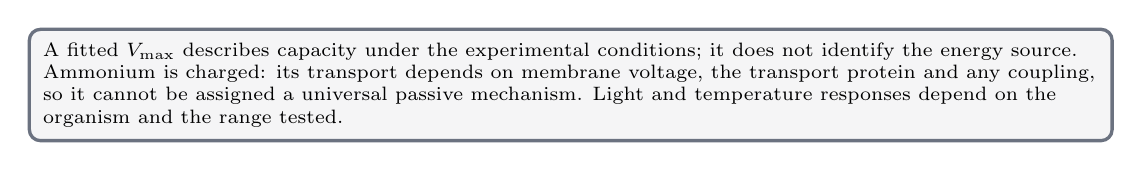
\begin{tikzpicture}[font=\scriptsize]
  \node[card=grey, text width=13.4cm, font=\scriptsize] {A fitted $V_\text{max}$ describes capacity under the experimental conditions; it does not identify the energy source. Ammonium is charged: its transport depends on membrane voltage, the transport protein and any coupling, so it cannot be assigned a universal passive mechanism. Light and temperature responses depend on the organism and the range tested.};
\end{tikzpicture}
\end{frame}

% pos 66
\begin{frame}{What sets the plateau?}
\twocol{
\begin{itemize}
  \item A saturating curve means some step has finite capacity
  \item Candidates: transporter abundance, transporter turnover, internal processing
  \item The plateau fits active or facilitated transport equally well
  \item At matched concentration and activity per unit surface, more active area per gram gives more uptake per gram
  \item Geometry alone does not set a universal $V_\text{max}$ or $K_s$
\end{itemize}}{
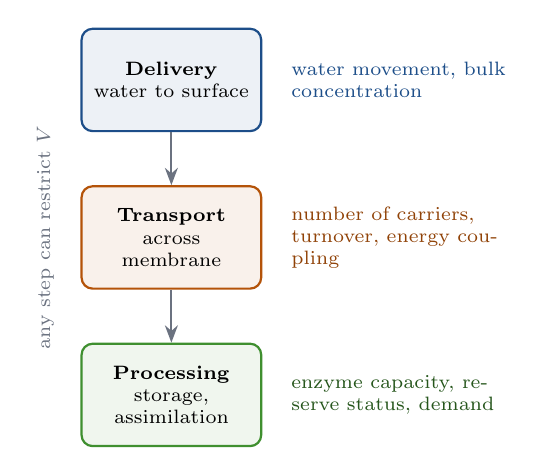
\begin{tikzpicture}[font=\scriptsize]
  \node[flow=sea, text width=2.0cm, minimum height=1.3cm] (d) at (0,2.4) {\textbf{Delivery}\\ water to surface};
  \node[flow=warm, text width=2.0cm, minimum height=1.3cm] (t) at (0,0.4) {\textbf{Transport}\\ across membrane};
  \node[flow=leaf, text width=2.0cm, minimum height=1.3cm] (p) at (0,-1.6) {\textbf{Processing}\\ storage, assimilation};
  \draw[arr] (d) -- (t); \draw[arr] (t) -- (p);
  \node[font=\scriptsize, sea, anchor=west, text width=2.8cm] at (1.4,2.4) {water movement, bulk concentration};
  \node[font=\scriptsize, warm!80!black, anchor=west, text width=2.8cm] at (1.4,0.4) {number of carriers, turnover, energy coupling};
  \node[font=\scriptsize, leaf!60!black, anchor=west, text width=2.8cm] at (1.4,-1.6) {enzyme capacity, reserve status, demand};
  \node[font=\scriptsize, grey, rotate=90] at (-1.6,0.4) {any step can restrict $V$};
\end{tikzpicture}
\fignote{Schematic.}}
\end{frame}

% pos 67
\begin{frame}{Three descriptions of a changing uptake rate}
\begin{center}
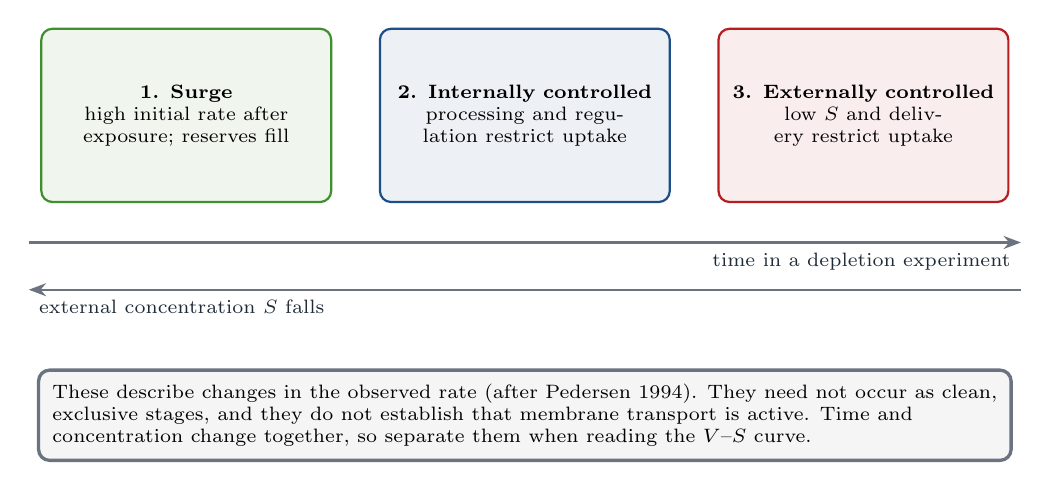
\begin{tikzpicture}[font=\scriptsize]
  \draw[arr] (0,0) -- (12.6,0) node[below left, font=\scriptsize, ink] {time in a depletion experiment};
  \draw[arr] (12.6,-0.6) -- (0,-0.6) node[below right, font=\scriptsize, ink] {external concentration $S$ falls};
  \node[flow=leaf, text width=3.4cm, minimum height=2.2cm, anchor=south] at (2.0,0.5) {\textbf{1. Surge}\\ high initial rate after exposure; reserves fill};
  \node[flow=sea, text width=3.4cm, minimum height=2.2cm, anchor=south] at (6.3,0.5) {\textbf{2. Internally controlled}\\ processing and regulation restrict uptake};
  \node[flow=hot, text width=3.4cm, minimum height=2.2cm, anchor=south] at (10.6,0.5) {\textbf{3. Externally controlled}\\ low $S$ and delivery restrict uptake};
  \node[card=grey, text width=12.0cm, font=\scriptsize, anchor=north] at (6.3,-1.6) {These describe changes in the observed rate (after Pedersen 1994). They need not occur as clean, exclusive stages, and they do not establish that membrane transport is active. Time and concentration change together, so separate them when reading the $V$–$S$ curve.};
\end{tikzpicture}
\end{center}
\end{frame}

% pos 68
\begin{frame}{The surge phase}
\twocol{
\begin{itemize}
  \item A transient high uptake rate soon after exposure
  \item Often seen in nutrient-depleted tissue
  \item Uptake temporarily exceeds assimilation into structural organic matter, so reserves accumulate
  \item Candidate mechanisms: reserve filling; feedback on transport or assimilation
  \item Occurrence and duration depend on prior conditions and the organism
\end{itemize}}{
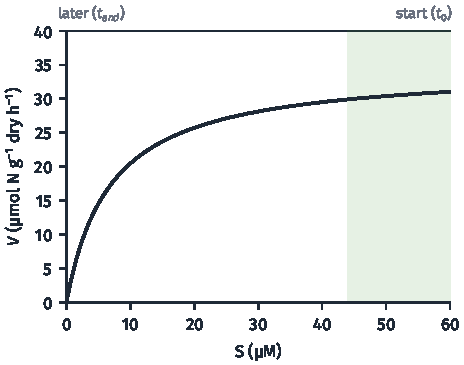
\includegraphics[width=0.95\linewidth]{fig_phase_surge}
\fignote{Shaded: high $S$ at the start of a depletion experiment. Curve: N-replete \textit{G. gracilis}, 15\,°C (Smit 2002, Table II).}}
\end{frame}

% pos 69
\begin{frame}{The internally controlled phase}
\twocol{
\begin{itemize}
  \item Internal processing and regulation restrict uptake while external delivery is sufficient
  \item Assimilation incorporates N into organic compounds
  \item Stored pools and nutrient demand feed back on further uptake
  \item A plateau does not identify one step (nitrate reductase, vacuole filling or another)
  \item Test internal N fractions and processing rates
\end{itemize}}{
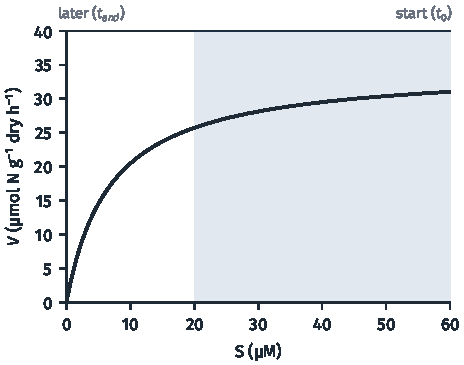
\includegraphics[width=0.95\linewidth]{fig_phase_internal}
\fignote{Shaded: concentrations where $V$ is near its limiting capacity. Curve as before (Smit 2002, Table II).}}
\end{frame}

% pos 70
\begin{frame}{The externally controlled phase}
\twocol{
\begin{itemize}
  \item In a closed vessel, uptake lowers the external concentration
  \item Low $S$ restricts uptake through less substrate at the transport sites
  \item External delivery through the boundary layer can restrict it too
  \item A low rate at low $S$ does not, by itself, prove diffusion limitation
  \item Test delivery by changing water movement
\end{itemize}}{
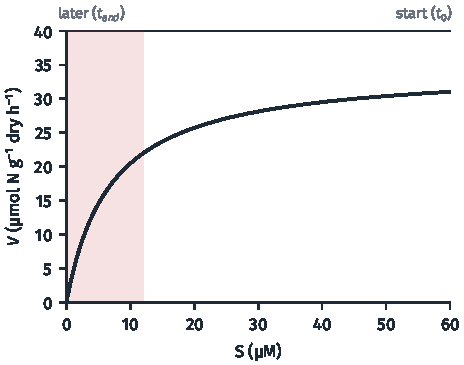
\includegraphics[width=0.95\linewidth]{fig_phase_external}
\fignote{Shaded: low $S$ late in a depletion experiment. Curve as before (Smit 2002, Table II).}}
\end{frame}

% pos 71
\begin{frame}{Delivery through the boundary layer}
\twocol{
\begin{itemize}
  \item Nutrients reach the surface by diffusion through the concentration boundary layer
  \item The flux rises with the bulk-to-surface concentration difference
  \item It falls as the effective layer thickness increases
  \item Relevant difference: bulk water to thallus surface, never seawater to total tissue N
  \item Two remedies: raise the bulk concentration, or increase water movement
\end{itemize}}{
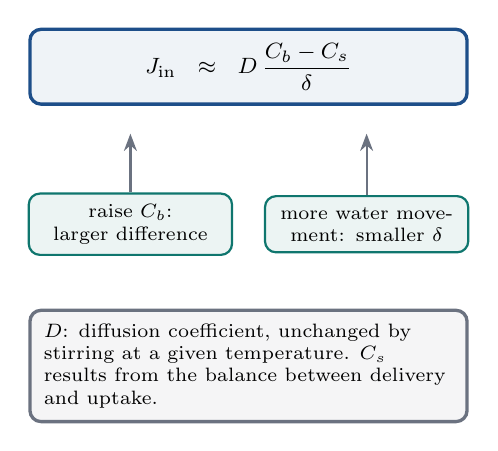
\begin{tikzpicture}[font=\scriptsize]
  \node[card=sea, text width=5.2cm, align=center] at (0,2.2) {\footnotesize $J_\text{in} \approx D\,\dfrac{C_b - C_s}{\delta}$};
  \node[flow=accent, text width=2.3cm, font=\scriptsize] (c) at (-1.5,0.2) {raise $C_b$:\\ larger difference};
  \node[flow=accent, text width=2.3cm, font=\scriptsize] (w) at (1.5,0.2) {more water movement: smaller $\delta$};
  \draw[arr] (c.north) -- (-1.5,1.35); \draw[arr] (w.north) -- (1.5,1.35);
  \node[card=grey, text width=5.2cm, font=\scriptsize] at (0,-1.6) {$D$: diffusion coefficient, unchanged by stirring at a given temperature. $C_s$ results from the balance between delivery and uptake.};
\end{tikzpicture}
\fignote{Planar layer, steady and approximately linear profile.}}
\end{frame}

% pos 72
\begin{frame}{Passive uptake}
\twocol{
\begin{itemize}
  \item Down the electrochemical gradient, with no energy coupling
  \item Simple diffusion through the lipid, or facilitated diffusion through a protein
  \item Small non-polar molecules (CO$_2$, O$_2$) cross the lipid directly
  \item Ions generally need membrane proteins
  \item NH$_3$ is uncharged; NH$_4^+$ is charged; their proportions depend on pH
  \item Protein-mediated ammonium uptake is well established
\end{itemize}}{
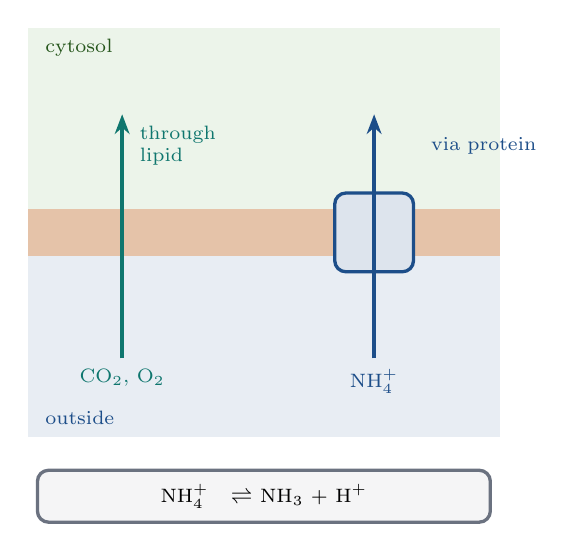
\begin{tikzpicture}[font=\scriptsize]
  \fill[sea!10] (-3.0,-2.6) rectangle (3.0,-0.3);
  \fill[leaf!10] (-3.0,0.3) rectangle (3.0,2.6);
  \fill[warm!35] (-3.0,-0.3) rectangle (3.0,0.3);
  \node[font=\scriptsize, sea, anchor=west] at (-2.9,-2.35) {outside};
  \node[font=\scriptsize, leaf!60!black, anchor=west] at (-2.9,2.35) {cytosol};
  \draw[very thick, accent, -{Stealth[length=2.5mm]}] (-1.8,-1.6) node[below, font=\scriptsize] {CO$_2$, O$_2$} -- (-1.8,1.5);
  \node[font=\scriptsize, accent, anchor=west, text width=1.3cm] at (-1.7,1.1) {through lipid};
  \node[draw=sea, very thick, fill=sea!15, rounded corners, minimum width=1.0cm, minimum height=1.0cm] at (1.4,0) {};
  \draw[very thick, sea, -{Stealth[length=2.5mm]}] (1.4,-1.6) node[below, font=\scriptsize] {NH$_4^+$} -- (1.4,1.5);
  \node[font=\scriptsize, sea, anchor=west, text width=1.4cm] at (2.0,1.1) {via protein};
  \node[card=grey, font=\scriptsize, text width=5.4cm, anchor=north, align=center] at (0,-3.0) {NH$_4^+ \rightleftharpoons$ NH$_3$ + H$^+$};
\end{tikzpicture}
\fignote{Schematic.}}
\end{frame}

% pos 73
\begin{frame}{Linear uptake responses}
\twocol{
\begin{itemize}
  \item A linear $V$–$S$ response gives a slope; report the tested range
  \item Do not extend the line indefinitely or read it as proof of simple diffusion
  \item A carrier well below saturation can also respond linearly
  \item A linear segment does not identify $V_\text{max}$ and $K_s$ separately
  \item At low $S$, $V \approx \alpha S$ with $\alpha = V_\text{max}/K_s$
\end{itemize}}{
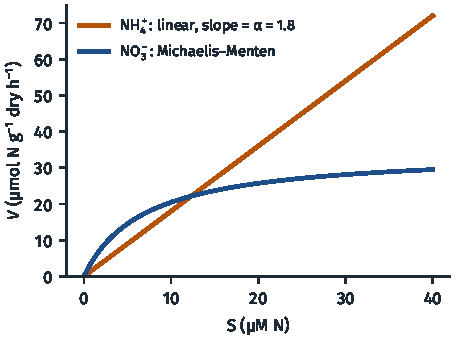
\includegraphics[width=0.95\linewidth]{fig_linear_vs_mm}
\fignote{N-replete \textit{Gracilaria gracilis} at 15\,°C: ammonium linear model, nitrate Michaelis–Menten model (Smit 2002, Tables I and II).}}
\end{frame}

% pos 74
\begin{frame}{Uptake, storage and growth}
\twocol{
\begin{itemize}
  \item Coupled: added nutrient produces an immediate growth response
  \item Luxury consumption: uptake exceeds immediate needs and fills reserves
  \item Growth can then lag behind uptake, and continue after supply falls
  \item High SA:V does not establish whether transport is passive or active
  \item Simple thallus form does not imply an absence of storage
\end{itemize}}{
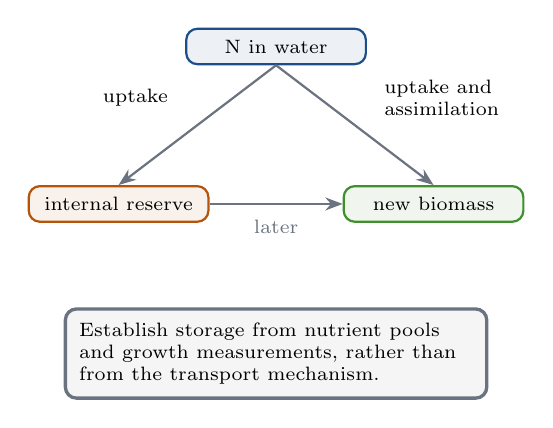
\begin{tikzpicture}[font=\scriptsize]
  \node[flow=sea, text width=2.0cm] (w) at (0,2.2) {N in water};
  \node[flow=warm, text width=2.0cm] (r) at (-2.0,0.2) {internal reserve};
  \node[flow=leaf, text width=2.0cm] (g) at (2.0,0.2) {new biomass};
  \draw[arr] (w.south) -- (r.north);
  \draw[arr] (w.south) -- (g.north);
  \node[font=\scriptsize, anchor=east] at (-1.25,1.55) {uptake};
  \node[font=\scriptsize, anchor=west, align=left] at (1.25,1.55) {uptake and\\ assimilation};
  \draw[arr] (r) -- node[below=2pt, font=\scriptsize] {later} (g);
  \node[card=grey, text width=5.0cm, font=\scriptsize] at (0,-1.7) {Establish storage from nutrient pools and growth measurements, rather than from the transport mechanism.};
\end{tikzpicture}
\fignote{Schematic.}}
\end{frame}

% pos 75
\begin{frame}{The Monod equation}
\twocol{
\begin{itemize}
  \item Describes \textbf{growth rate} as a saturating function of external substrate
  \item Same mathematical form as Michaelis–Menten; different response variable and parameters
  \item Assumes growth tracks the external supply
  \item Fits poorly where luxury consumption decouples growth from uptake
  \item Neither curve identifies the membrane mechanism
\end{itemize}}{
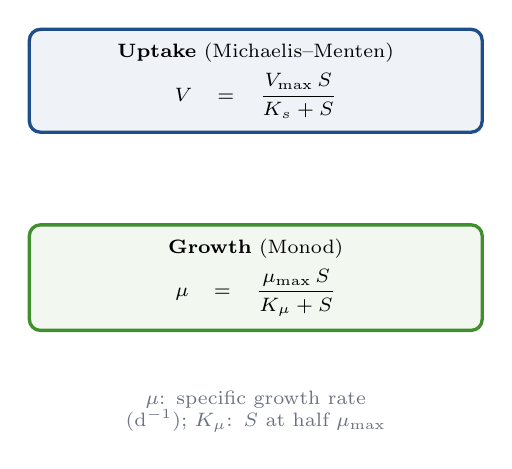
\begin{tikzpicture}[font=\scriptsize]
  \node[card=sea, text width=5.4cm, align=center] at (0,1.6) {\textbf{Uptake} (Michaelis–Menten)\\[3pt] $V = \dfrac{V_\text{max}\,S}{K_s + S}$};
  \node[card=leaf, text width=5.4cm, align=center] at (0,-0.9) {\textbf{Growth} (Monod)\\[3pt] $\mu = \dfrac{\mu_\text{max}\,S}{K_\mu + S}$};
  \node[font=\scriptsize, grey, text width=5.4cm, align=center] at (0,-2.6) {$\mu$: specific growth rate (d$^{-1}$); $K_\mu$: $S$ at half $\mu_\text{max}$};
\end{tikzpicture}}
\end{frame}

% pos 76
\begin{frame}{Facilitated uptake}
\twocol{
\begin{itemize}
  \item A form of \textbf{passive} transport: down the electrochemical gradient
  \item A membrane protein provides the route
  \item Carriers use \textbf{alternating access}: open outside, occluded, open inside
  \item Channels provide a pore instead
  \item Carriers can be selective, saturate and be inhibited; these do not make transport active
\end{itemize}}{
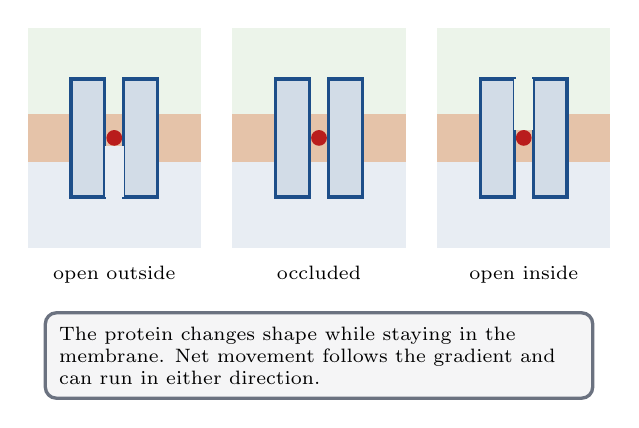
\begin{tikzpicture}[font=\scriptsize, x=1cm, y=1cm]
  \foreach \x/\lab/\o/\i in {-2.6/open outside/1/0, 0/occluded/0/0, 2.6/open inside/0/1}{
    \fill[warm!35] (\x-1.1,-0.3) rectangle (\x+1.1,0.3);
    \fill[sea!10] (\x-1.1,-1.4) rectangle (\x+1.1,-0.3);
    \fill[leaf!10] (\x-1.1,0.3) rectangle (\x+1.1,1.4);
    \draw[very thick, sea, fill=sea!20] (\x-0.55,-0.75) rectangle (\x-0.12,0.75);
    \draw[very thick, sea, fill=sea!20] (\x+0.12,-0.75) rectangle (\x+0.55,0.75);
    \ifnum\o=1 \fill[sea!10] (\x-0.12,-0.75) rectangle (\x+0.12,-0.1); \fi
    \ifnum\i=1 \fill[leaf!10] (\x-0.12,0.1) rectangle (\x+0.12,0.75); \fi
    \fill[hot] (\x,0) circle (0.1);
    \node[font=\scriptsize, anchor=north] at (\x,-1.5) {\lab};
  }
  \node[card=grey, text width=6.6cm, font=\scriptsize, anchor=north] at (0,-2.2) {The protein changes shape while staying in the membrane. Net movement follows the gradient and can run in either direction.};
\end{tikzpicture}
\fignote{Schematic carrier cycle.}}
\end{frame}

% pos 77
\begin{frame}{Biphasic uptake}
\twocol{
\begin{itemize}
  \item A concentration response with distinguishable behaviour over different ranges
  \item At low $S$: a steep, saturating component dominates
  \item At higher $S$: uptake keeps rising more slowly
  \item One description: the sum of a saturating and an approximately linear component
  \item Both components operate at the same time in this description
\end{itemize}}{
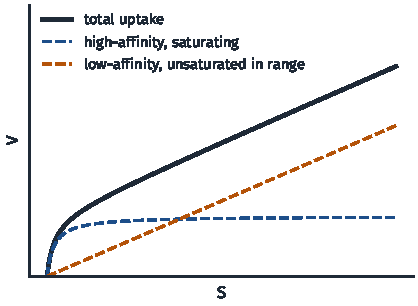
\includegraphics[width=0.95\linewidth]{fig_biphasic}
\fignote{Schematic with illustrative parameters.}}
\end{frame}

% pos 78
\begin{frame}{Describing a biphasic curve}
\begin{center}
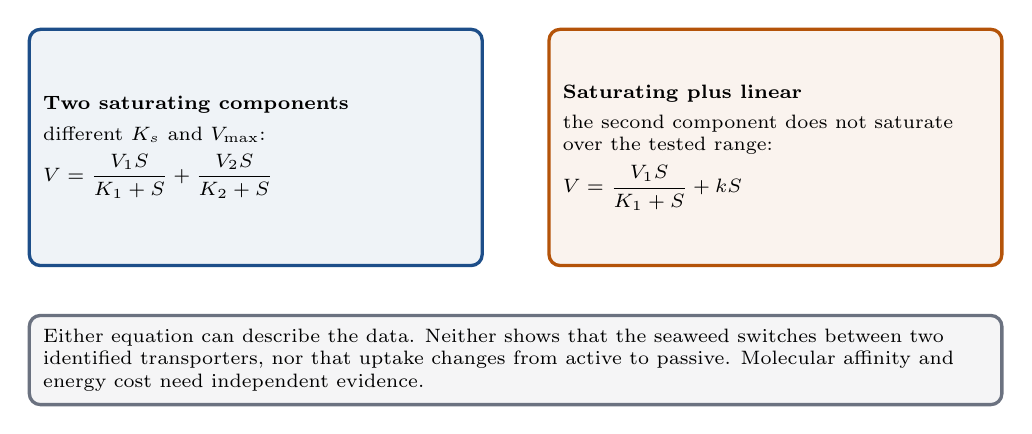
\begin{tikzpicture}[font=\scriptsize]
  \node[card=sea, text width=5.4cm, minimum height=3.0cm] (a) at (-3.3,0) {\textbf{Two saturating components}\\[3pt] different $K_s$ and $V_\text{max}$:\\[3pt] $V = \dfrac{V_1 S}{K_1 + S} + \dfrac{V_2 S}{K_2 + S}$};
  \node[card=warm, text width=5.4cm, minimum height=3.0cm] (b) at (3.3,0) {\textbf{Saturating plus linear}\\[3pt] the second component does not saturate over the tested range:\\[3pt] $V = \dfrac{V_1 S}{K_1 + S} + kS$};
  \node[card=grey, text width=12.0cm, font=\scriptsize] at (0,-2.7) {Either equation can describe the data. Neither shows that the seaweed switches between two identified transporters, nor that uptake changes from active to passive. Molecular affinity and energy cost need independent evidence.};
\end{tikzpicture}
\end{center}
\end{frame}

% pos 79
\begin{frame}{Interpreting a biphasic response}
\twocol{
\begin{itemize}
  \item Nutritional history can change the measured response
  \item So can external delivery, multiple pathways and regulation
  \item Use the fitted pattern to generate competing predictions
  \item Then test them with independent evidence
\end{itemize}}{
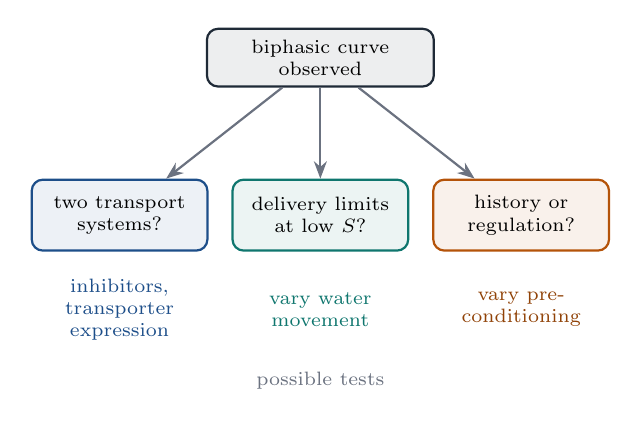
\begin{tikzpicture}[font=\scriptsize]
  \node[flow=ink, text width=2.6cm] (o) at (0,2.2) {biphasic curve observed};
  \node[flow=sea, text width=1.95cm, minimum height=0.9cm, font=\scriptsize] (h1) at (-2.55,0.2) {two transport systems?};
  \node[flow=accent, text width=1.95cm, minimum height=0.9cm, font=\scriptsize] (h2) at (0,0.2) {delivery limits at low $S$?};
  \node[flow=warm, text width=1.95cm, minimum height=0.9cm, font=\scriptsize] (h3) at (2.55,0.2) {history or regulation?};
  \draw[arr] (o) -- (h1); \draw[arr] (o) -- (h2); \draw[arr] (o) -- (h3);
  \node[font=\scriptsize, sea, text width=2.1cm, align=center] at (-2.55,-1.0) {inhibitors, transporter expression};
  \node[font=\scriptsize, accent, text width=2.1cm, align=center] at (0,-1.0) {vary water movement};
  \node[font=\scriptsize, warm!80!black, text width=2.1cm, align=center] at (2.55,-1.0) {vary pre-conditioning};
  \node[font=\scriptsize, grey] at (0,-1.9) {possible tests};
\end{tikzpicture}
\fignote{Schematic.}}
\end{frame}

% pos 80
\begin{frame}{Three shapes of the uptake response}
\begin{center}
\begin{tikzpicture}[font=\scriptsize]
\foreach \i/\t/\f/\c in {0/Linear/{0.9*x}/warm, 1/Hyperbolic/{9*x/(2+x)}/sea, 2/Biphasic/{6*x/(1+x)+0.35*x}/ink}{
\begin{axis}[at={(\i*4.6cm,0)}, width=4.6cm, height=3.5cm, xmin=0, xmax=10, ymin=0, ymax=10,
  axis lines=left, xtick=\empty, ytick=\empty, xlabel={\footnotesize $S$}, ylabel={\footnotesize $V$}, title={\scriptsize\textbf{\t}}]
  \addplot[very thick, \c, domain=0:10, samples=80] {\f};
\end{axis}}
\end{tikzpicture}
\end{center}
{\footnotesize
\begin{itemize}
  \item Hyperbolic: rises and saturates; the usual Michaelis–Menten description
  \item Linear: no saturation within the tested range
  \item Biphasic: distinguishable behaviour over different concentration ranges
  \item None of the three, on its own, identifies the transport mechanism
\end{itemize}}
\fignote{Schematic curves.}
\end{frame}

% pos 81
\begin{frame}{Factors modifying uptake rates}
\begin{center}
\begin{tikzpicture}[font=\scriptsize]
  \node[flow=ink, text width=2.8cm, minimum height=1.1cm] (v) at (0,0) {\textbf{uptake rate $V$}\\ and its kinetics};
  \foreach \p/\t/\c in {{(0,2.15)}/{water movement\\ (boundary layer)}/sea, {(4.3,1.1)}/{nutrient form\\ (NO$_3^-$, NH$_4^+$)}/accent, {(4.3,-1.1)}/{nutritional\\ history}/warm, {(0,-2.15)}/{light and\\ photoperiod}/sand, {(-4.3,-1.1)}/{temperature}/hot, {(-4.3,1.1)}/{SA:V and\\ thallus form}/leaf}{
    \node[flow=\c, text width=2.8cm, minimum height=1.1cm, font=\scriptsize] (n) at \p {\t};
    \draw[arr] (n) -- (v);
  }
\end{tikzpicture}
\end{center}
\fignote{These influences interact. State which one an experiment changes, and which measurements separate its effect from the others.}
\end{frame}

% pos 82
\begin{frame}{Water movement}
\twocol{
\begin{itemize}
  \item Kinetic studies usually vary $S$; water movement also changes $V$
  \item Flow thins the concentration boundary layer, shortening the diffusion distance
  \item Advection and mixing replenish depleted water near the thallus
  \item The diffusion coefficient itself need not change
  \item Faster flow can raise $C_s$ and still increase uptake, because $\delta$ shrinks more
\end{itemize}}{
\begin{tikzpicture}[font=\scriptsize]
  \foreach \y/\d/\lab/\c in {1.6/1.1/slow flow: thick layer/grey, -1.4/0.4/fast flow: thin layer/sea}{
    \fill[leaf!35] (-3,\y-0.25) rectangle (3,\y+0.25);
    \fill[\c!30] (-3,\y+0.25) rectangle (3,\y+0.25+\d);
    \draw[\c, dashed] (-3,\y+0.25+\d) -- (3,\y+0.25+\d);
    \node[font=\scriptsize, \c, anchor=west] at (-3,\y-0.5) {\lab};
  }
  \foreach \x in {-2,0,2}{\draw[-{Stealth[length=2mm]}, grey] (\x-0.4,3.3) -- (\x+0.2,3.3);}
  \foreach \x in {-2,0,2}{\draw[-{Stealth[length=2mm]}, very thick, sea] (\x-0.6,-0.45) -- (\x+0.6,-0.45);}
  \node[font=\scriptsize, leaf!60!black] at (2.4,1.6) {thallus};
  \node[font=\scriptsize, leaf!60!black] at (2.4,-1.4) {thallus};
\end{tikzpicture}
\fignote{Schematic: shaded band is the depleted concentration boundary layer.}}
\end{frame}

% pos 83
\begin{frame}{Water movement changes the low-concentration response}
\twocol{
\begin{itemize}
  \item Nitrate uptake by \textit{G. gracilis} on a shaker at 0, 250 and 500 oscillations min$^{-1}$
  \item More water movement: lower apparent $K_s$ and steeper initial slope
  \item Consistent with improved delivery at low bulk concentration
  \item Shaking does not raise the molecular diffusion coefficient
  \item The shaker setting is a treatment, not a measured velocity at the thallus
\end{itemize}}{
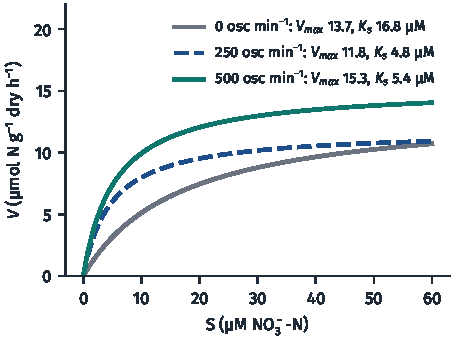
\includegraphics[width=0.95\linewidth]{fig_water_motion}
\fignote{Model curves from Smit (2002), Table III; $V_\text{max}$ in µmol N g$^{-1}$ dry h$^{-1}$.}}
\end{frame}

% pos 84
\begin{frame}{Nutritional history}
\begin{center}
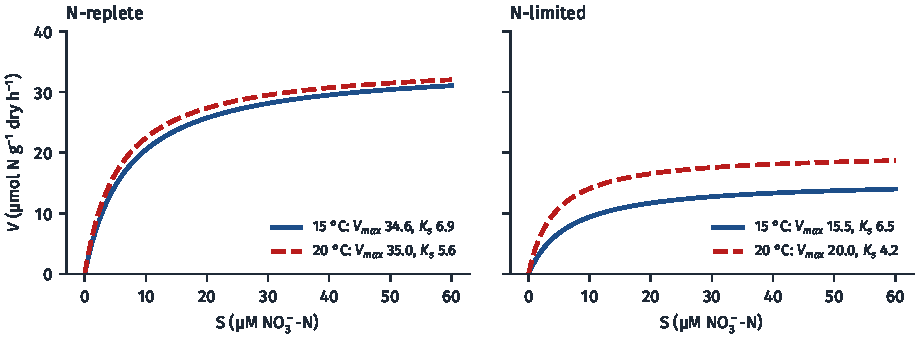
\includegraphics[width=0.86\textwidth]{fig_nutritional_history}
\end{center}
\vspace{-4pt}
{\footnotesize Nitrate uptake by \textit{Gracilaria gracilis} grown N-replete or N-limited, at 15 and 20\,°C. Prior nutrient exposure changes the curve; each parameter difference needs its own statistical test.}
\fignote{Model curves from Smit (2002), Table II; $V_\text{max}$ in µmol N g$^{-1}$ dry h$^{-1}$, $K_s$ in µM.}
\end{frame}

% pos 85
\begin{frame}{Nutritional history changes uptake}
\twocol{
\begin{itemize}
  \item Prior exposure changes internal reserves, demand and uptake properties
  \item Depleted but functional tissue may acquire N faster than replete tissue
  \item Prolonged deprivation or damage can also reduce capacity
  \item In \textit{G. gracilis}, the ammonium slope rose with N limitation
  \item Linear does not mean passive; saturating does not mean active
\end{itemize}}{
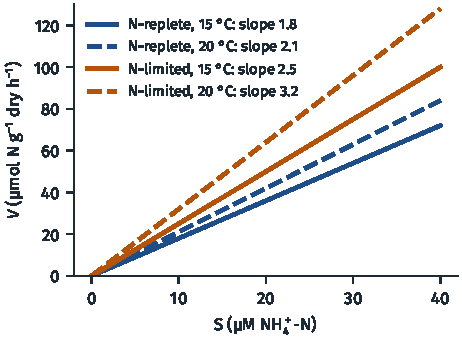
\includegraphics[width=0.95\linewidth]{fig_nh4_linear}
\fignote{Linear models for ammonium uptake by \textit{Gracilaria gracilis} (Smit 2002, Table I); lines drawn through the origin from the reported slopes.}}
\end{frame}

% pos 86
\begin{frame}{Light environment}
\twocol{
\begin{itemize}
  \item Photosynthesis supplies energy (ATP), reductant and carbon skeletons
  \item These support N assimilation into amino acids, proteins and nucleic acids
  \item Light can affect nutrient demand, transport regulation and assimilation
  \item At low irradiance, more light may enhance these processes
  \item Saturation, photoinhibition or another limiting resource can change the response at higher irradiance
\end{itemize}}{
\begin{tikzpicture}[font=\scriptsize]
  \node[flow=sand, text width=2.0cm] (l) at (0,2.6) {light};
  \node[flow=leaf, text width=2.6cm] (p) at (0,1.2) {photosynthesis};
  \node[flow=warm, text width=1.5cm, font=\scriptsize] (e) at (-2.0,-0.2) {ATP, reductant};
  \node[flow=warm, text width=1.5cm, font=\scriptsize] (c) at (2.0,-0.2) {carbon skeletons};
  \node[flow=sea, text width=3.6cm] (a) at (0,-1.6) {N assimilation: NO$_3^-$ $\rightarrow$ NO$_2^-$ $\rightarrow$ NH$_4^+$ $\rightarrow$ amino acids};
  \draw[arr] (l) -- (p); \draw[arr] (p) -- (e); \draw[arr] (p) -- (c); \draw[arr] (e) -- (a); \draw[arr] (c) -- (a);
  \node[font=\scriptsize, grey, text width=5.4cm, align=center] at (0,-2.75) {Glucose contains C, H and O, but no N or P.};
\end{tikzpicture}
\fignote{Schematic.}}
\end{frame}

% pos 87
\begin{frame}{Photoperiod}
\twocol{
\begin{itemize}
  \item Nitrate reductase: NO$_3^-$ $\rightarrow$ NO$_2^-$; nitrite reductase: NO$_2^-$ $\rightarrow$ NH$_4^+$
  \item Nitrate reductase activity and synthesis can show a daily rhythm
  \item Photoperiod can therefore affect nitrate uptake and assimilation
  \item Uptake and assimilation need not stop at once in darkness: stored carbon and energy support them
  \item Track uptake and assimilation separately; their difference changes the reserve
\end{itemize}}{
\begin{tikzpicture}[font=\scriptsize]
  \fill[sand!35] (0,0) rectangle (3.2,0.5);
  \fill[ink!80] (3.2,0) rectangle (6.4,0.5);
  \node[font=\scriptsize] at (1.6,0.25) {day};
  \node[font=\scriptsize, white] at (4.8,0.25) {night};
  \draw[very thick, sea] (0,1.0) .. controls (1.0,2.6) and (2.2,2.6) .. (3.2,2.0) .. controls (4.0,1.6) and (5.4,1.5) .. (6.4,1.4);
  \draw[very thick, leaf, dashed] (0,1.0) .. controls (1.0,2.0) and (2.2,2.1) .. (3.2,1.8) .. controls (4.0,1.4) and (5.4,1.2) .. (6.4,1.1);
  \node[font=\scriptsize, sea, anchor=west] at (0.1,2.9) {uptake};
  \node[font=\scriptsize, leaf!60!black, anchor=west] at (1.6,1.15) {assimilation};
  \draw[arr] (0,0.6) -- (0,3.2) node[above, font=\scriptsize, ink] {rate};
\end{tikzpicture}
\fignote{Schematic, not data.}}
\end{frame}

% pos 88
\begin{frame}{Temperature}
\twocol{
\begin{itemize}
  \item Affects transport, metabolism and growth over process- and species-specific ranges
  \item Warming can raise a rate below its optimum and reduce it above
  \item $Q_{10}$ = rate at $T+10$ ÷ rate at $T$
  \item $Q_{10}$ = 2: a doubling over that interval only
  \item Two temperatures cannot locate an optimum
  \item Control external delivery when testing temperature effects on uptake
\end{itemize}}{
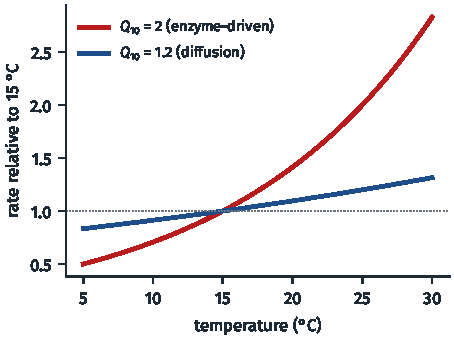
\includegraphics[width=0.95\linewidth]{fig_q10}
\fignote{Illustration only: each curve holds $Q_{10}$ constant from 5 to 30\,°C. Real responses peak and decline above an optimum.}}
\end{frame}

% pos 89
\begin{frame}{Different forms of DIN}
\twocol{
\begin{itemize}
  \item Ammonium and nitrate differ in transport, regulation and assimilation
  \item In some studies, ammonium uptake does not saturate over the tested range
  \item Other models are then needed to describe it
  \item Neither a linear nor a saturating response identifies the mechanism
  \item Use electrochemical gradients and evidence about energy coupling
\end{itemize}}{
\footnotesize
\renewcommand{\arraystretch}{1.35}
\begin{tabular}{@{}>{\raggedright\arraybackslash}p{1.85cm}>{\raggedright\arraybackslash}p{1.95cm}>{\raggedright\arraybackslash}p{3.3cm}@{}}
 & \textbf{NH$_4^+$} & \textbf{NO$_3^-$}\\\hline
best model & linear & Michaelis–Menten\\
parameters & slope 1.8–3.2 & $V_\text{max}$ 15.5–35.0\\
 & & $K_s$ 4.2–6.9 µM\\
N-limited & steeper slope & lower $V_\text{max}$\\\hline
\end{tabular}
\fignote{\textit{Gracilaria gracilis}, 15 and 20\,°C (Smit 2002, Tables I and II). Slope in µmol N g$^{-1}$ dry h$^{-1}$ per µM; $V_\text{max}$ in µmol N g$^{-1}$ dry h$^{-1}$.}}
\end{frame}

% pos 90
\begin{frame}{Ammonium and nitrate uptake by \textit{Gracilaria gracilis}}
\begin{columns}[t,onlytextwidth]
\begin{column}{0.49\textwidth}\centering
{\footnotesize\textbf{Ammonium: linear}}\\
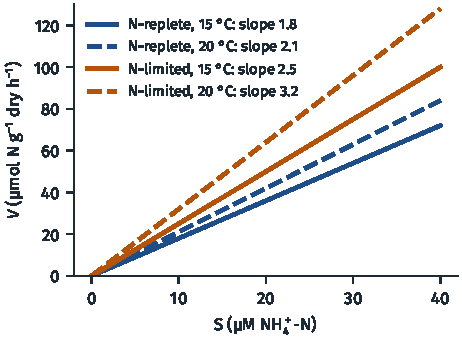
\includegraphics[width=0.95\linewidth]{fig_nh4_linear}
\end{column}
\begin{column}{0.49\textwidth}\centering
{\footnotesize\textbf{Nitrate: saturating}}\\
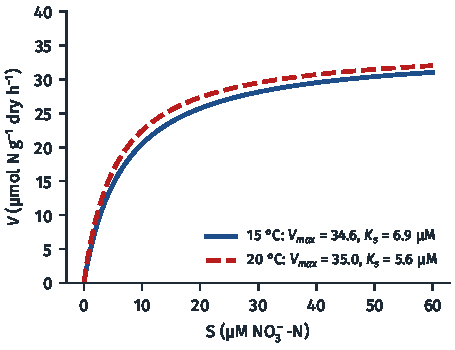
\includegraphics[width=0.95\linewidth]{fig_mm_nitrate}
\end{column}
\end{columns}
\fignote{Model curves from Smit (2002), Tables I and II. Lines are drawn across the concentration range tested; do not extend them beyond it.}
\end{frame}

% pos 91
\begin{frame}{Interaction: ammonium and nitrate}
\twocol{
\begin{itemize}
  \item N-limited \textit{G. gracilis} given 50 µM nitrate and 25 µM ammonium together
  \item NO$_3^-$ uptake reduced by up to 38\,\% in the presence of NH$_4^+$ above ca.\ 5 µM
  \item Suppression lasted 30–35 min, until ammonium fell below that concentration
  \item Then nitrate uptake increased
  \item Nutrients interact: measure them together
\end{itemize}}{
\begin{tikzpicture}[font=\scriptsize]
  \draw[arr] (0,0) -- (6.2,0) node[below left, font=\scriptsize, ink] {time};
  \fill[hot!12] (0,0) rectangle (2.4,3.6);
  \node[font=\scriptsize, hot, align=center] at (1.2,3.3) {NH$_4^+$ $>$ 5 µM};
  \draw[very thick, warm] (0,2.8) .. controls (1.0,1.6) and (1.8,0.6) .. (2.4,0.35) -- (6.0,0.15);
  \node[font=\scriptsize, warm, anchor=west] at (2.6,0.65) {NH$_4^+$ in medium};
  \draw[very thick, sea] (0,1.2) -- (2.4,1.2) .. controls (2.8,1.2) and (2.9,2.0) .. (3.4,2.0) -- (6.0,2.0);
  \node[font=\scriptsize, sea, anchor=west] at (3.5,2.3) {NO$_3^-$ uptake rate};
  \node[font=\scriptsize, grey, anchor=north] at (2.4,0) {30–35 min};
\end{tikzpicture}
\fignote{Schematic of the pattern reported by Smit (2002), Figure 7.}}
\end{frame}

% pos 92
\begin{frame}{Other factors affecting uptake}
\twocol{
\begin{itemize}
  \item SA:V explains much of the variation among species, within a species, and among parts of one thallus
  \item Hyaline hairs alter local chemistry and boundary layers; they do not establish higher intrinsic affinity
  \item Reproduction can raise nutrient demand
  \item Older, slower-growing tissue may take up less
  \item Life-history phases and genotypes can differ in uptake
\end{itemize}}{
\begin{tikzpicture}[font=\scriptsize]
  \node[flow=ink, text width=2.2cm] (v) at (0,0) {\textbf{uptake}};
  \foreach \p/\t/\c in {{(0,2.15)}/{SA:V and form}/leaf, {(2.7,1.15)}/{hyaline hairs}/accent, {(2.7,-1.15)}/{reproductive state}/warm, {(0,-2.15)}/{thallus age}/grey, {(-2.7,-1.15)}/{life-history phase, genotype}/sea, {(-2.7,1.15)}/{desiccation, nutrients, competition}/hot}{
    \node[flow=\c, text width=2.05cm, minimum height=0.95cm, font=\scriptsize] (n) at \p {\t};
    \draw[arr] (n) -- (v);
  }
\end{tikzpicture}
\fignote{Hyaline hairs: Lichtenberg et al. (2017).}}
\end{frame}

\end{document}
